
\documentclass[12pt,a4paper]{article}

%% Language and font encodings
\usepackage[french, english]{babel}

\usepackage[utf8x]{inputenc}
\usepackage[T1]{fontenc}
\usepackage{footnote}
\usepackage{pgfplots}
\usepackage{tikz}
\usepackage{multicol}
\usepackage{diagbox}
\usepackage{float}
\usepackage{lastpage}
\usepackage{array}
\usepackage{fancyhdr}
\usepackage[english]{fancyref}
\usepackage[UKenglish]{datetime}
\usepackage{pdfpages}
%\usepackage{todonotes}
\usepackage{placeins}
%% Sets page size and margins
\usepackage[a4paper,top=3cm,bottom=2cm,left=3cm,right=1cm,marginparwidth=1.75cm]{geometry}
\pgfplotsset{width=10cm,compat=1.9}
\setlength{\columnsep}{0.3cm}
\pagestyle{fancy}
\cfoot{Page \thepage \hspace{1pt} of \pageref{LastPage}}

%% Useful packages
\usepackage{amsmath}
\usepackage{graphicx}
\definecolor{titlepagecolor}{cmyk}{0,0,0,0}
\definecolor{namecolor}{cmyk}{1,1,1,1}
\usepackage{subcaption}
\usepackage[colorinlistoftodos]{todonotes}
\usepackage[colorlinks=true, allcolors=black]{hyperref}
\usepackage{wrapfig}
\usepackage{listings}
\usepackage{xcolor}
\renewcommand{\thefigure}{\arabic{section}.\arabic{figure}}
%\renewcommand{\thetable}{\arabic{section}.\arabic{figure}}

\definecolor{mGreen}{rgb}{0,0.6,0}
\definecolor{mGray}{rgb}{0.5,0.5,0.5}
\definecolor{mPurple}{rgb}{0.58,0,0.82}
\definecolor{backgroundColour}{rgb}{0.99,0.99,0.99}

\lstdefinestyle{CStyle}{
	backgroundcolor=\color{backgroundColour},   
	commentstyle=\color{mGreen},
	keywordstyle=\color{magenta},
	numberstyle=\tiny\color{mGray},
	stringstyle=\color{mPurple},
	basicstyle=\footnotesize,
	breakatwhitespace=false,         
	breaklines=true,                 
	captionpos=b,                    
	keepspaces=true,                 
	numbers=left,                    
	numbersep=5pt,                  
	showspaces=false,                
	showstringspaces=false,
	showtabs=false,                  
	tabsize=2,
	language=C
}
\lstdefinestyle{Bashstyle}{
	backgroundcolor=\color{backgroundColour},   
	commentstyle=\color{mGreen},
	keywordstyle=\color{magenta},
	numberstyle=\tiny\color{mGray},
	stringstyle=\color{mPurple},
	breakatwhitespace=false,         
	breaklines=true,                 
	captionpos=b,                    
	keepspaces=true,                                                 
	showspaces=false,                
	showstringspaces=false,
	showtabs=false,                  
	tabsize=2,
	language=bash
}
\lstdefinestyle{PyStyle}{
	backgroundcolor=\color{backgroundColour},   
	commentstyle=\color{mGreen},
	keywordstyle=\color{magenta},
	numberstyle=\tiny\color{mGray},
	stringstyle=\color{mPurple},
	basicstyle=\footnotesize,
	breakatwhitespace=false,         
	breaklines=true,                 
	captionpos=b,                    
	keepspaces=true,                 
	numbers=left,                    
	numbersep=5pt,                  
	showspaces=false,                
	showstringspaces=false,
	showtabs=false,                  
	tabsize=2,
	language=Python
}
\lstset{
	basicstyle=\ttfamily,
	columns=fullflexible,
	showstringspaces=false,
	commentstyle=\color{gray}\upshape
}

\lstdefinelanguage{XML}
{
	morestring=[b]",
	morestring=[s]{>}{<},
	morecomment=[s]{<?}{?>},
	numberstyle=\tiny\color{mGray},       
	breaklines=true, 
	numbers=left,            
	numbersep=5pt,       
	identifierstyle=\color{mGreen},
	keywordstyle=\color{magenta},
	morekeywords={xmlns,version,type}% list your attributes here
}
%\usepackage{natbib}
\pagestyle{fancy}
\title{Development and study of ailerons vs. twisting wing}
\author{\large{Negretto Didier Chérubin, MT-MA-3}}
\makeindex

\begin{document}
	\date{\today}
\begin{titlepage}
\newgeometry{top=3cm,bottom=2cm,left=2cm,right=2cm,marginparwidth=1.75cm}
\hspace{+2.8cm} %defines the geometry for the titlepage
\pagecolor{titlepagecolor}
\noindent
\begin{center}

\includegraphics[width=8cm]{fig/EPFL_Logo_Digital_RGB_PROD.jpg}\\[-1em]
\color{black}
\par
\noindent
\hspace{-30cm}
\makebox[3pt][l]{\rule{19 cm}{1pt}}
\par
\noindent
\textbf{\Large \textsf{Biorobotics laboratory}}\\
\end{center}
\vspace{0.5cm}
\hspace{-3.5cm}
	\begin{figure}[H]
    	\centering
		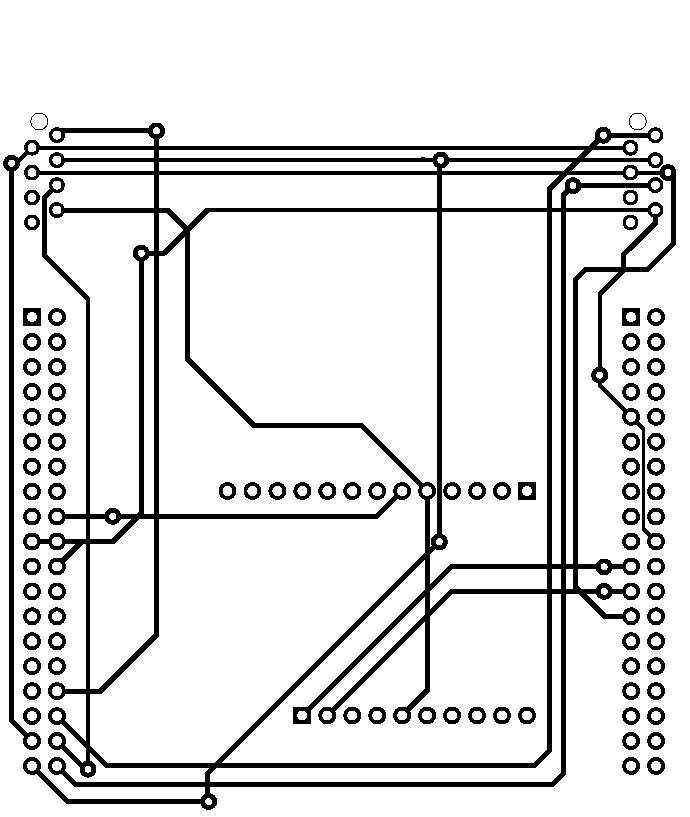
\includegraphics[width=12 cm]{fig/front.pdf}
	\end{figure}

\vfill


\hspace{+0.5cm}
{\huge \huge \textsf{MOUSE TREADMILL CONTROL}}

\vskip\baselineskip
\noindent
\hspace{+3.5cm}
{\textsf{\today}
\vskip\baselineskip
\noindent
\hspace{+3.5cm}
{\textsf{By \textbf{\Large{Didier Chérubin Negretto} }}}
\vskip\baselineskip
\noindent
\hspace{+3.5cm}
{\textsf{Professor: \large\textbf{Auke Ijspeert}}}
\vskip\baselineskip
\noindent
\hspace{+3.5cm}
{\textsf{Assistant :\textbf{Shravan Tata Ramalingasetty} }}
}
\end{titlepage}

\restoregeometry % restores the geometry
\nopagecolor% Use this to restore the color pages to white
\begin{center}
\chead{\textit{\textbf{Mouse treadmill control}}}
%\newpage
\textbf{\Large{Semester project description}}\\
\end{center}
\begin{multicols}{2}
[]

\paragraph{Objectives and preliminary considerations} 
\lfoot{\today}
\rfoot{Biorobotics laboratory}
\begin{figure}[H]
	\centering
	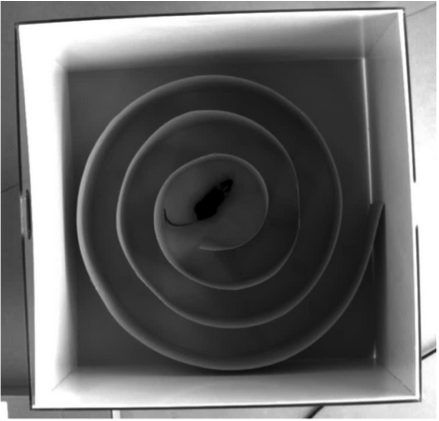
\includegraphics[width=0.9\linewidth]{fig/OleSetup}
	%\includegraphics[width=\linewidth]{fig_sim/fin_comp}
	\caption{Roll coefficient as a function of the angle of attack for different values of twisting and folding angles. Schematics of folding configurations are added. }\label{fig:tw_vs_fold_bar}
\end{figure}
The project consists of designing and manufacturing the electronics and control for a mouse treadmill. After that the system is characterized and tested. This work starts from \cite{Ole}: in this paper a cardboard maze is used to test the mouse behaviour. This setup is quite simple and comes with some drawbacks (i.e. it is not possible to analyse the mouse gait or control its speed and direction), which are addressed by the treadmill design. The new design features closed-loop speed control, a user interface (with real-time plotting), data logging, moreover the system can be expanded easily thanks to the use of MAVLink.

\paragraph{System architecture}
 For the system architecture one $\mu$controller is used for the closed-loop control. This controller sends and receives data using a USB cable and the UART 232 protocol with the MAVLink messaging protocol. On the other side the PC can get the messages, log them and plot them. To measure the speed of the treadmill two optical sensors are used. These sensors are the same that can be found in gaming mouse. The sensors provide rich information which can be used not only to measure the speed of the surface of the treadmill, but also the estimate the quality of the measure itself. By using this information the control loop is aware of possible measuring problems and can therefore discard low quality information.\\
 Finally, to ease the user experience, a cross-platform graphical user interface as well as documentation, unit tests and a user manual are provided. 
 
\paragraph{Testing and results}
Once the system is built some tests are carried out to characterize the system performances.
First the noise at 0 [$\frac{m}{s}$] in the sensors is measured, then the noise at constant speed. This is important to determine what type of noise is present in the system and whatever it useful to filter it and how. The quality of the surface with a static and moving treadmill is also compared. The noise is characterize with the following parameters: \todo{ADD RESULTS}
Then one test on the step response is performed, which gave these results: \todo{ADD RESULTS}
Finally the treadmill was tested using a sinusoidal routine and the tracking performances (the difference between the desired path and the real routine) are shown in figure \ref{fig:track_res}.

\paragraph{Cost}
As a prof of concept the treadmill seems to be a proper solution providing solutions to many of the drawbacks of the previous cardboard maze setup. On the other hand not all the requirements are fulfilled yet, some improvements may include: new motors, which can provide the required speed and torque for better tracking and a camera to get information on the mouse position so that experiments with a free moving mouse can be performed as well. The main drawbacks of this design are the increased complexity, the increased cost and the need of a fixed-head mouse. No need to underline that the much richer information that can be retrieved using the new design as well as the possibility to solve the issue of the fixed-head mouse in future iterations of this design outfaces all the drawbacks.  



\end{multicols}

\clearpage
\lfoot{ }
\rfoot{ }
\chead{ }
%\begin{abstract}

%\end{abstract}

\pagestyle{plain}
\clearpage

\tableofcontents
\clearpage
\pagestyle{fancy}
\section{Introduction}\label{sec:intro}
In this section the main objectives and the state of the art for the project are presented as well as the overall structure of this report.
\subsection{Motivation}
\begin{wrapfigure}{L}{0.42\textwidth}
	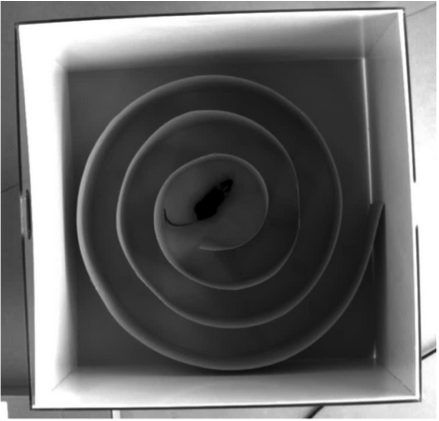
\includegraphics[width=\linewidth]{fig/OleSetup.png}
	\caption{The experimental setup used in \cite{Ole}.}\label{fig:OleSetup}
	\vspace{-2 cm}
\end{wrapfigure}
The studies on mammal locomotion have driven more and more attention over the years, and especially experiments on mice, such as \cite{Ole}, have enhanced our understanding of the neuronal circuits that enable locomotion. The experimental setup in \cite{Ole}, on the other hand, is quite rudimental. As shown in \ref{fig:OleSetup} it only consist in a spiral maze made out cardboard. This setup comes with some advantages such as:
\begin{itemize}
	\item Low price
	\item Simple to implement and use
	\item Untrained mice can be employed
	\item Free moving mouse
\end{itemize}
As well as some disadvantages:
\begin{itemize}
	\item Impossibility to analyse the mouse gait
	\item The mouse movements can't be imposed
\end{itemize}
To asses these issues a new design is needed for conducting such experiments. The new platform needs to allow the control on the walking surface on which the mouse is standing in such a way that a specific speed profile can be imposed to the mouse. Moreover it must be possible to analyse the mouse gait using cameras. \\
For the new design inspiration is taken from some existing solutions on the market. 
\subsection{Requirements}
First the mechanical requirements are discussed and stated. Table \ref{tab:Requirements} summarizes them.
\begin{table}[H]
	\centering
	\begin{tabular}{l||c|r} 
		\textbf{Description}&\textbf{Value}  &\textbf{Unit}  \\ 
		\hline
		\hline 
		Dimensions of the moving surface & 0.5 & $[m^2]$ \\ 
		\hline 
		Course & $\infty$  & $[m]$  \\ 
		\hline 
		Maximum speed & 3 & $[\frac{m}{s}]$ \\ 
		\hline 
		Maximum acceleration & 2 & $[\frac{m}{s^2}]$  \\ 
		\hline 
		Position resolution & 0.01 & $[m]$  \\ 
		\hline 
		Speed resolution & 0.02  & $[\frac{m}{s}]$  \\ 
		\hline 
		Maximum weight & 0.1  & $[kg]$  \\  
		\hline 
		Mounting time for 1 person & 30 & $[min]$  \\
		\hline 
		Maximum weight of the mouse & 40  & $[g]$ \\
		\hline 
		Length of common experiment (distance, time) & (20, 600)  & ($[m]$,$[s]$)  \\
	\end{tabular} 
	\caption{Summary of the requirements for the mouse treadmill platform.}
	\label{tab:Requirements}
\end{table}
The functional requirements are listed as well:
\begin{itemize}
	\item \textbf{Closed-loop control} Once a 2D speed setpoint is chosen the speed of the surface needs to be measured and the motor control signal need to be adjusted automatically to reach the desired setpoint. 
	\item \textbf{Speed routines} The user can define a speed routine, which needs to be executed by the treadmill. The speed routine consist in a list of 2D speed setpoints and the time interval during which the machine should execute them.
	\item \textbf{User interface} The user can use a Graphical user interface (GUI) on a computer to be able to use the mouse treadmill. This interface informs the user if the sensors are correctly connected and initialized, and it should give a live update of the treadmill speed.
	\item \textbf{Data logging} The user can save the data sent by the treadmill during the experiment for future uses. 
	\item \textbf{Expandability of the system} The user can easily expand the system with other controllers to have other features, than the ones listed above.
\end{itemize}

\subsection{Structure of the report}
This report is structured as follows: an introduction is given in section \ref{sec:intro}, the system architecture and communication are explained in \ref{sec:archi}. Section \ref{sec:design}, describes the design decisions and the components choices made .Section \ref{sec:control} describes the control strategy and shows some preliminary responses.
Finally in section \ref{sec:conc} the conclusion of the project is given. The code, code documentation as well as the data-sheets of the components are annexed.

\section{System architecture} \label{sec:archi}
In this section the architecture of the system is explained and detailed.
One first overview of the system is given in figure \ref{fig:arch}.
\begin{figure}[H]
	\centering
	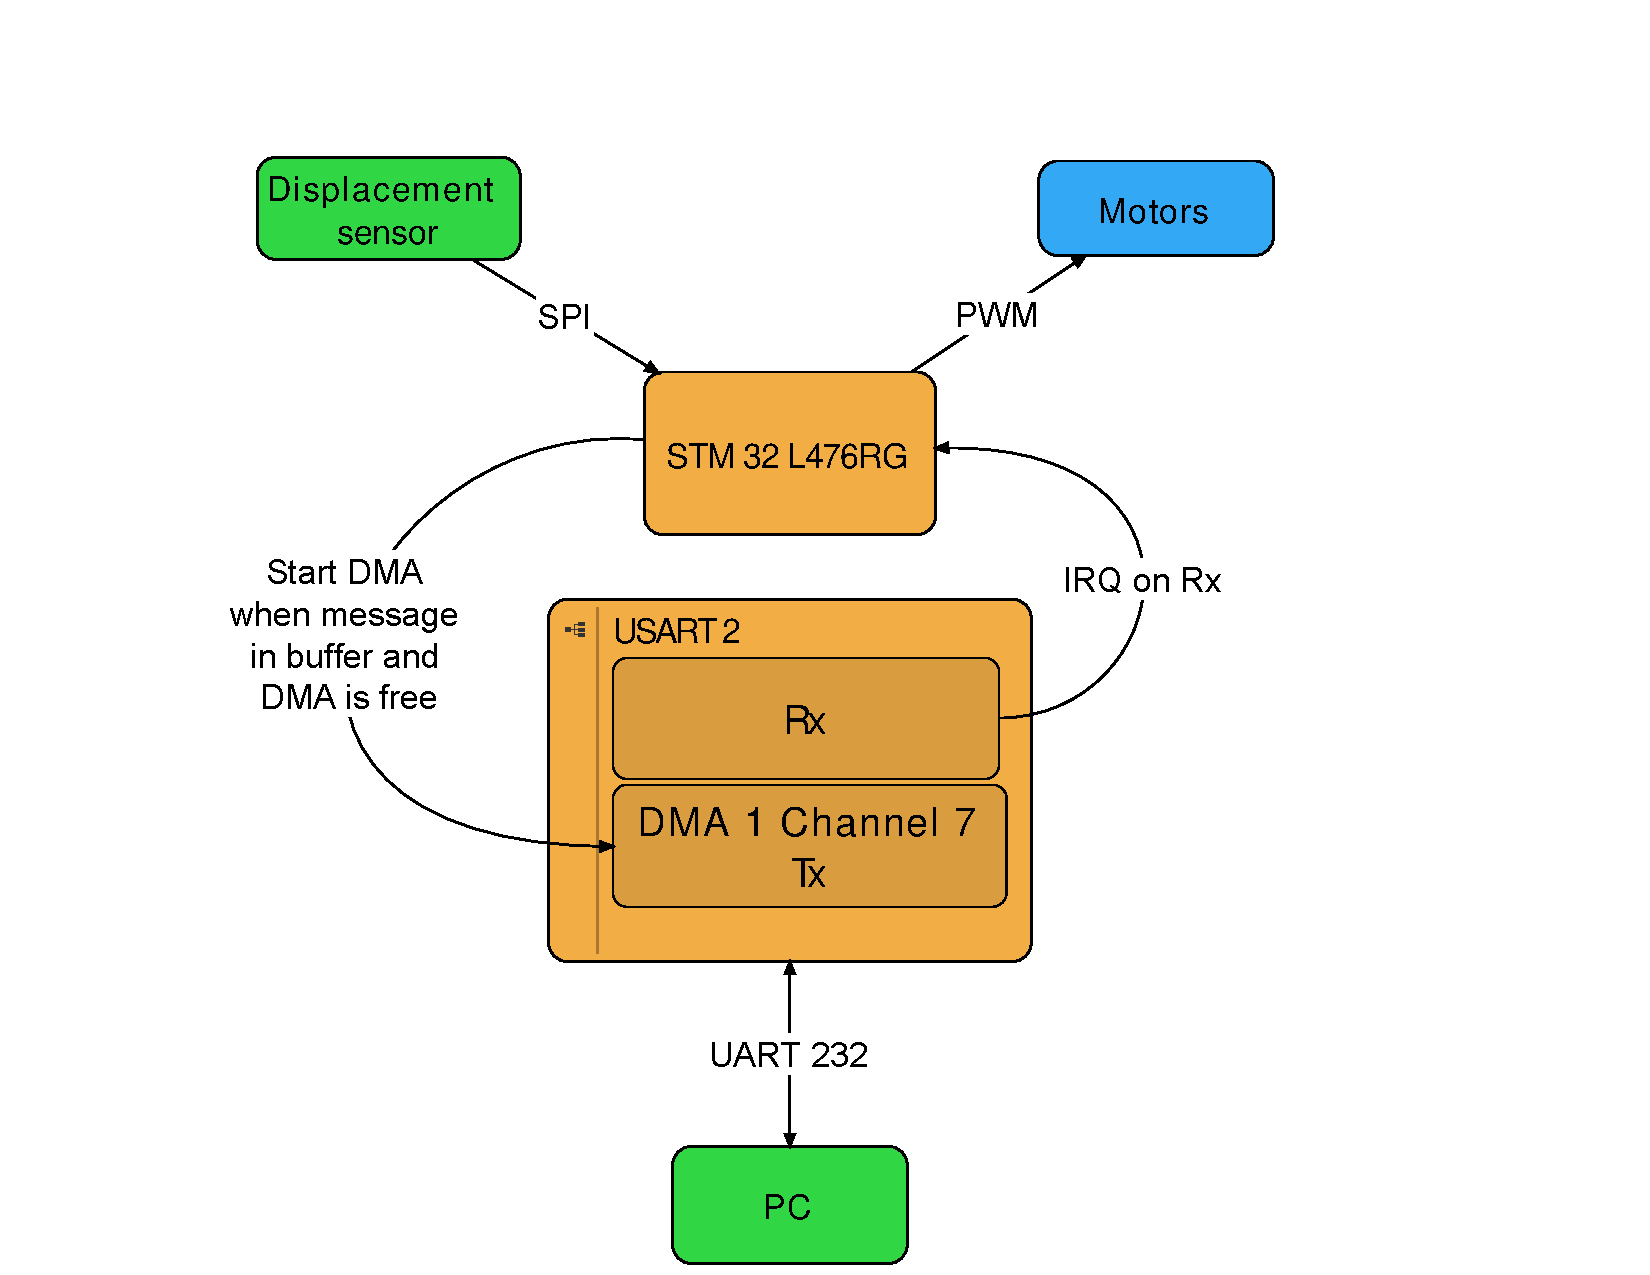
\includegraphics[width=0.9\linewidth]{fig/archi.pdf}
	\caption{Architecture for mouse treadmill project}
	\label{fig:arch}
\end{figure}
The core of the system is the STM32L476RG, which can read from the sensors using the SPI interface and control the motors using the PWM. Moreover it can communicate with the computer and the GUI for data logging and to receive the inputs form the user. The communication with the computer uses the DMA capabilities of the microcontroller to free the processor from waiting for the communication to end before being able to take care of other tasks.

\section{Design choices}\label{sec:design}
In this section the design choices are explained and justified. First the choice of the board is analysed, then the sensors and finally the calculations for the motor dimensioning are shown.
\subsection{Board}
For the board choice different types are taken into account:
\begin{itemize}
	\item \textbf{Single board computer}: In this category the raspberry pi and the odroid are taken into consideration. These boards offer powerful computers, which can be running operating systems such as Linux or Windows, which makes them interesting. Unfortunately they can't provide any accurate timing,  which is needed for the motor control and PWM generation.
	\item \textbf{Evaluation boards}: In this category the STM32 nucleo boards as well as the arduino boards can be found. These boards allow proper timing of the signals and accurate PWM generation, but on the other hand a computer is needed for plotting and storing the data, which can't be done locally on the board due to memory restrictions and limited resources on the board.
\end{itemize}
Due to the constraints in the system the second category is consider for implementation, the STM32L476RG board is taken for the system. Table \ref{tab:board} summarizes the features of the board.
\begin{table}[H]
	\centering
	\begin{tabular}{l||c|r} 
		\textbf{Description}&\textbf{Value}  &\textbf{Unit}  \\ 
		\hline
		\hline 
		Architecture & ARM-Cortex 32-bit with FPU & $-$ \\ 
		\hline 
		Clock frequency & 80  & $[MHz]$  \\ 
		\hline 
		Flash memory & 1 & $[MB]$ \\ 
		\hline 
		RAM memory & 128 & $[KB]$  \\ 
		\hline 
		I2C interfaces & 3 & $-$  \\ 
		\hline 
		USART interfaces & 5  & $-$  \\ 
		\hline 
		SPI interfaces & 3  & $-$  \\  
		\hline 
		DMA controller & 14 & $-$  \\
		\hline
		Cost & 20.58 &$[CHF]$
	\end{tabular} 
	\caption{STM32L476RG main features.}
	\label{tab:board}
\end{table}
One of the most important feature of the board is the DMA, which enhances the performances of the CPU. The DMA is used for the UART communication with the computer. This technique frees the CPU from waiting for the UART communication to be finished, so that it can spend more time on other activities. This same solution can be, in principle, adopted for the SPI communication if a standard SPI is used. Unfortunately the timing diagrams for the sensors are not standard, thus some time needs to be "wasted" by the processor so that the sensors can keep up with the communication.
Other interesting features are: the big flash memory, the good RAM memory and the low cost. One drawback is that dynamic memory allocation is not possible in such an small system to prevent stack overflow and problems during run time. This is why the size of the speed routine is limited to a given number of points.
Finally the multiple serial interfaces allow the possibility to expand the system to a bigger one with more controllers involved.

\subsection{Communication}
\todo{ADD Baud rate, and other specs of the communication}

\begin{wrapfigure}{R}{0.42\textwidth}
	
\includegraphics[width=\linewidth]{fig/MAVLink_logo.png}
	\caption{MAVLink logo}\label{fig:MAVLink_logo}
\end{wrapfigure}
For the communication with the computer the UART protocol is chosen. This choice is almost mandatory since most boards are provided with an UART to USB interface and a mini-USB connector. The STM32L476RG is no exception to this rule. The main settings for the UART protocol are reported in table \ref{tab:UART}.

\begin{table}[H]
	\centering
	\begin{tabular}{l||c|r} 
		\textbf{Parameter} &\textbf{Value} &\textbf{Unit}\\ 
		\hline
		\hline 
		Baud rate & 230400 & [$\frac{Bits}{s}$] \\ 
		\hline 
		Word length & 8 & [$Bits$] \\ 
		\hline 
		Parity & None & $-$\\ 
		\hline 
		Stop bits & 1 & [$Bits$]\\ 
		\hline 
		MSB first & Disable & $-$  \\ 
	\end{tabular} 
	\caption{Table describing the main parameters of the UART communication protocol.}
	\label{tab:UART}
\end{table}

Since the system needs to be expanded for future more complex experiments some thought is put in the choice of the messaging protocol to allow this key feature.
The best solution found is MAVLink. "MAVLink is a very lightweight messaging protocol for communicating with drones"\cite{mavlink}, one can say that the mouse treadmill is not meant to fly around, but this messaging protocol is flexible enough to be adapted to the mouse treadmill.
More precisely a dialect is described in \ref{app:mavlink}, and summarized in table \ref{tab:msg}. Thanks to the description file it is possible to generate libraries in different programming languages (C, Python, Java, ...) and if in the future a new message is required a additional definition can be added to the file and the libraries can be regenerated.

Despite the light weight MAVLink comes with some interesting features, such is high reliability (detects packets drops and corruption), high efficiency (only 14-bits of overhead), it can also allow up to 255 concurrent systems on the network.

\begin{table}[H]
	\centering
	\begin{tabular}{l||p{3cm}|l|l|l} 
		\textbf{Name} &\textbf{Description} &\textbf{Sender} &\textbf{Receiver} & \textbf{Type}\\ 
		\hline
		\hline 
		HEARTBEAT &Verifies communication& STM32 & PC & Status \\ 
		\hline 
		SPEED\_INFO &Measured speed  & STM32 & PC & Info \\ 
		\hline 
		SPEED\_SETPOINT & Speed setpoint & PC/STM32 & STM32/PC & Status\\ 
		\hline 
		MODE\_SELECTION & Changes mode & PC & STM32 & $-$\\ 
		\hline 
		MOTOR\_SETPOINT & Up time of PWM duty cycle & STM32 & PC & Info  \\ 
		\hline 
		POINT\_LOADED & Acknowledge for routine point loaded  & STM32 & PC & $-$ \\ 
		\hline 
		POINT & Information for one point of the routine  & PC & STM32 & $-$  \\  
		\hline 
		ERROR & Error message & STM32 & PC & $-$  \\
		\hline
		RAW\_SENSOR & Raw sensor values & STM32 & PC & Status\\
	\end{tabular} 
	\caption{List and description of the MAVLink messages. The Type indicates whatever the message is high frequency (Info), low frequency (Status) or none of the previous ones ($-$)}
	\label{tab:msg}
\end{table}

\subsection{Sensor}
For sensing the speed of the wheel a contactless solution is chosen. To achieve this goal a optical gaming mouse sensor is taken. Nevertheless the sensor need to come mounted on a PCB with a simple interface to reduce the time needed to design and manufacture the machine.
Because of that the PMW3360 is chosen for the implentation.
The working principle of the sensor is quite simple. The sensor is equipped with a LED to light a given area and a camera. The camera takes picture of the moving surface with a frequency of up to 12000 $[fps]$. Using the integrated DSP module some features are extracted form the images and, by knowing the displacement of the features, it is possible to determine how much the surface has moved on the X and Y direction.
Some other useful information can be retrieved from the sensor such as :
\begin{itemize}
	\item \textbf{Lift status} This bit in the motion register gives information about the status of the sensor and especially if the sensor detects a surface or not. This information is used to determine if the read value is valid or not.
	\item \textbf{Surface quality (SQUAL)} This register gives an information about how many features are detected on the surface. This value is used to verify the quality of the measurement, which is considered valid only if the number of detected feature is above a given threshold.
	\item \textbf{SROM ID} This value is read after the power up of the sensor to verify that the SROM of the sensor is uploaded correctly using the SPI interface. If this value is not as expected it means that the sensor is not initialized correctly and thus might not work properly. 
\end{itemize}
The performances of the sensor are summarized on table \ref{tab:PMW3360}\footnote{$[cpi]$ stands for counts per inch.}. For more details refer to \ref{app:PMW3660}.
\begin{table}[H]
	\centering
	\begin{tabular}{l||c|r} 
		\textbf{Description}&\textbf{Value}  &\textbf{Unit}  \\ 
		\hline
		\hline 
		High speed detection & 6.3 & $[\frac{m}{s}]$ \\ 
		\hline 
		High acceleration detection & 490  & $[\frac{m}{s^2}]$  \\ 
		\hline 
		Default resolution & 5000 & $[cpi]$ \\ 
		\hline 
		Resolution error of & 1 & $[\%]$  \\ 
		\hline 
		4 wires SPI interface & 1 & $-$  \\ 
		\hline
		Cost & 29.99 &$[\$]$
	\end{tabular} 
	\caption{PMW3660 main features.}
	\label{tab:PMW3360}
\end{table}


\subsection{Motor}
To properly dimension the motors these assumptions are taken:
\begin{multicols}{2}[]
\begin{enumerate}
	\item $\eta = 1$ No losses in wheel-sphere coupling
	\item No slip of the wheel on the sphere
	\item Hollow sphere
	\item Flat disk
\end{enumerate}
\end{multicols}
The data given are
\begin{multicols}{2}[]
\begin{itemize}
	\item $m_s$ mass of the sphere
	\item $r_s$ radius of the sphere
	\item $m_w$ mass of the wheel
	\item $r_w$ radius of the wheel
	\item $M_{max}$ maximum torque provided by the motor-gearbox 
	\item $\omega_{max}$ maximum angular speed of the motor-gearbox
	\item $J_m$ inertia of the rotor
\end{itemize}
\end{multicols}
It is therefore possible to estimate the maximum continuous  acceleration and speed of the sphere.

\section{Control} \label{sec:control}
In this section the main aspect of the control are discussed as well as some results.
For the closed-loop control a simple PI controller is used (see \ref{sec:controller}). This can be improved in future works to allow for faster and better performance control. The implementation of the controller is done in CodeSTM32/mouseDrive.c in the function void mouseDriver\_control\_idle(void). 

\subsection{Inputs/Outputs}
In this section the signal definitions are described.
The control diagram is shown in figure \ref{fig:ctrl_diag}. The signals are defined as follow:
\begin{figure}[H]
	\centering
	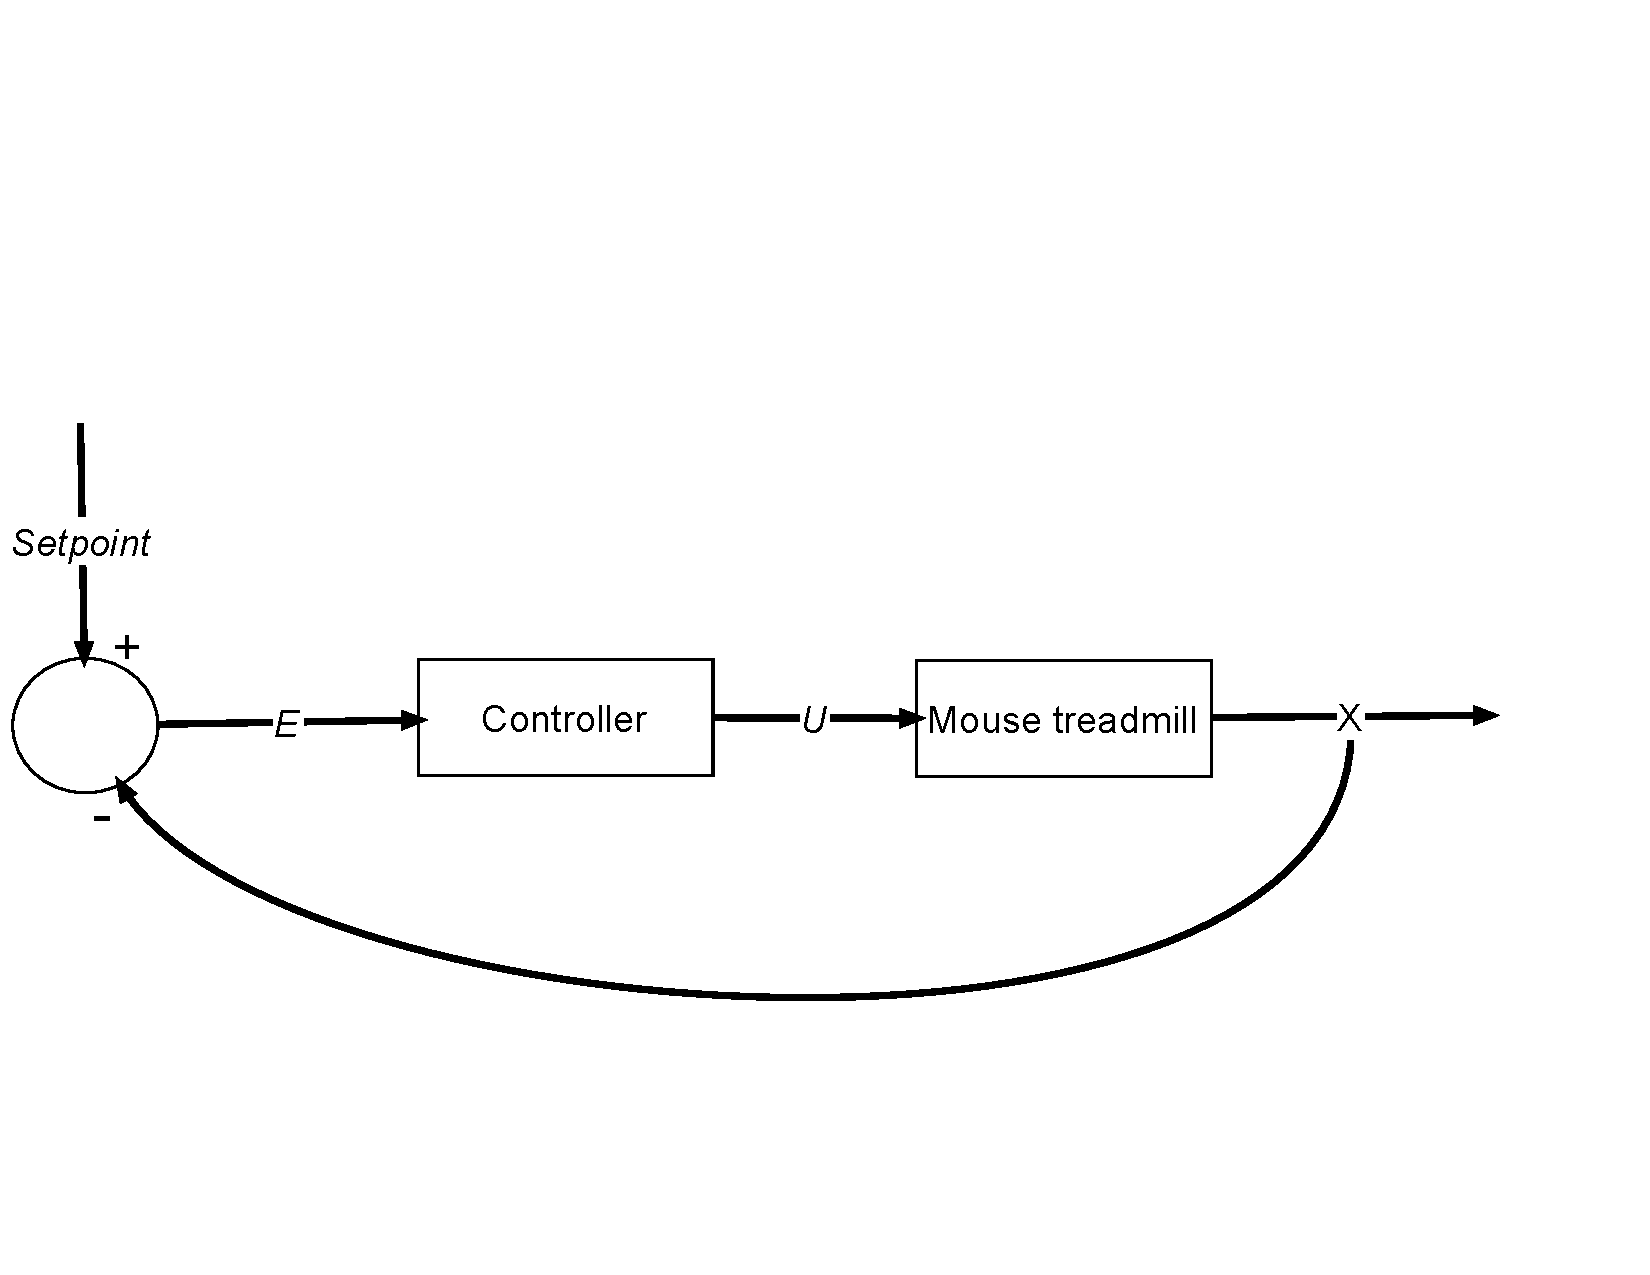
\includegraphics[width=0.8\linewidth]{fig/ctrl_diag.pdf}
	\caption{Control diagram}\label{fig:ctrl_diag}
\end{figure}

\begin{itemize}
	\item 
	$X = \begin{bmatrix}
	v_x\\
	v_y
	\end{bmatrix}$
	: is the measured $v_x$ and $v_y$ speeds. This measure is done using the optical sensors, which means that the raw values are as defined in the datasheet of the sensors (see \ref{app:PMW3660}). In short words the sensor runs a navigation program, which does the correlation between two images as fast as possible and finds out of how many counts the two images are displaced in the $x$ and $y$ direction of the sensor, those values are then integrated up to when the motion burst is performed. Since two sensors are used, only one axis of each sensor is meaningful for the control (since the other one is always fixed). The information that can be retrieved from one sensor is the number of counts along one axis that the ball has done since the last read. This can then be translated in to meters by knowing the resolution of the sensor (which is given in counts per inch) and the relation between inches and meters. Furthermore the speed can be computed by keeping track of when the last measure is taken, and the actual time, thus knowing the $dt$ between two measures.
	\item	
	$E = \begin{bmatrix}
	e_x\\
	e_y
	\end{bmatrix}$: is the error id est the difference between the setpoint and the measured speed
	\item  
	$U = 
	\begin{bmatrix}
		u_x\\
		u_y
	\end{bmatrix}$: is the control signal, which is the up time of the duty cycle of the PWM signal controlling the X and Y directions. The parameters of this signal can be modified by using the PRESCALER\_PWM and COUNTER\_PERIOD\_PWM. This two values allow for defining the frequency and number of possible values of the PWM signal.
\end{itemize}
\subsection{Controller} \label{sec:controller}
In this section the internal structure of the controller is described.
The inputs in the controller are the errors on the speed setpoint in X and Y. The control signal is defined as in equation \ref{eq:U}.
\begin{equation}\label{eq:U}
U = 
\begin{bmatrix}
u_x\\
u_y
\end{bmatrix}
= K * 
\begin{bmatrix}
e_x\\
e_y
\end{bmatrix} + I *
\begin{bmatrix}
i_x\\
i_y
\end{bmatrix} 
\end{equation}
Where $K$ and $I$ are constant scalar values and $\begin{bmatrix}i_x\\i_y\end{bmatrix}$ is a vector containing the sum of the errors over all the past measures where the motor signal $U$ is not the maximum allowed. This condition is taken to avoid wind up and overshoot in the controller.\\
Moreover the control is done only if the measures taken are valid. Which means that the SQUAL measure is bigger than SQUAL\_THRESH, the sensors are not lifted, and the PRODUCT\_ID is equal 66.
If those conditions are met it means that the surface quality is good, the sensor "sees" correctly the surface and the communication is done correctly.
If the measures are not valid for more than MAX\_MISSING\_MEASURES the motors are stopped and the mode goes to STOP mode to avoid damage to the machine.
\subsection{Results}
In this section the results of the control are shown as well as the achieved performances in terms measures \ref{sec:measure_test} and control \ref{sec:control_test}.
\subsubsection{Measure test}\label{sec:measure_test}
In this section a simple experiment is described and the results are shown. First the zero speed noise is measured in the sensors, then the same measure is repeated while spinning the ball at constant speed. This let us characterize the noise in the sensors and decide whatever some filtering is required.

\subsubsection{Control test}\label{sec:control_test}
In this section the $I$ and $K$ parameters in equation \ref{eq:U} are tuned, then the step responses are measured. Finally a 2D routine is described and the tracking error is analysed to see whatever the machine is able to follow such a routine and with which performances.








\section{Conclusion} \label{sec:conc}

\newpage
\section[User manual]{User manual for mouse treadmill software}
The software is well documented in the docs folder, nevertheless some important things are pointed out in this report so that the user can more easily install and start using the mouse treadmill. The installation guide for the PC software, a user manual for the GUI, a explanation on how to write a speed routine as well as a guide on how to expand the system with new messages is provided. Note that all the provided commands and instructions are tested for MAC, mavlink is available also for LINUX and WINDOWS, the user can adapt these command to be able to install and successfully use the software on his machine. 
\subsection{Installation of the PC software}\label{sec:install}
First python 3 needs to be installed, for that see \cite{py}. GIT needs to be install as well. Some other python packages needs to be installed, they can be obtained using PiP. The required ones are:\\
\begin{multicols}{3}[]
	\begin{itemize}
		\item pyserial
		\item os
		\item sys
		\item numpy
		\item appjar
		\item tqdm
		\item json
		\item matplotlib
	\end{itemize}
\end{multicols}

Make sure that pymavlink is not install. This is important since the dialect used is not a standard one, but it is custom. Do not install pymavlink using PiP.\\

To install the software the sequent steps have to be accomplished:
\begin{enumerate}
	\item Clone the git repository of the project using 
	\begin{lstlisting}[style = Bashstyle]
	$ git clone https://github.com/DidierNegretto/3DMouseTreadmill.git
	\end{lstlisting}
	\item Move inside the repository
	\begin{lstlisting}[style = Bashstyle]
	$ cd 3DMouseTreadmill/
	\end{lstlisting}
	\item Make sure no previous version of pymavlink is installed
	\begin{lstlisting}[style = Bashstyle]
	$ pip uninstall pymavlink
	\end{lstlisting}
	\item Remove the mavlink directory
	\begin{lstlisting}[style = Bashstyle]
	$ rm -r -f mavlink/
	\end{lstlisting}
	\item Clone the mavlink repository
	\begin{lstlisting}[style = Bashstyle]
	$ git clone https://github.com/mavlink/mavlink.git
	\end{lstlisting}
	\item Update the submodule
	\begin{lstlisting}[style = Bashstyle]
	$ git submodule update --init --recursive
	\end{lstlisting}
	\item Copy mouse.xml file and the mouse.py files into mavlink/pymavlink/dialects/v20 
	\item Change directory to mavlink/
	\begin{lstlisting}[style = Bashstyle]
	$ cd mavlink
	\end{lstlisting}
	\item Export the path to the repository so that python will find all the code it needs to run
	\begin{lstlisting}[style = Bashstyle]
	$ export PYTHONPATH=`path_to_repository/3DMouseTreadmill/`
	\end{lstlisting}
	\item Change directory to pymavlink
	\begin{lstlisting}[style = Bashstyle]
	$ cd pymavlink
	\end{lstlisting}
	\item Setup everything using the setup.py provided
	\begin{lstlisting}[style = Bashstyle]
	$ python3 setup.py install --user
	\end{lstlisting}
	
\end{enumerate}
\subsection{How to use the GUI}  
In this section the use of the GUI and its functionalities are described.
First of all the GUI provided can be expanded using the functions in the mouse.py generated using mavlink, and thus can be improved for future versions of the project. One screenshot of the GUI is shown in figure \ref{fig:GUI}.
\begin{figure}[htp]
	\centering
	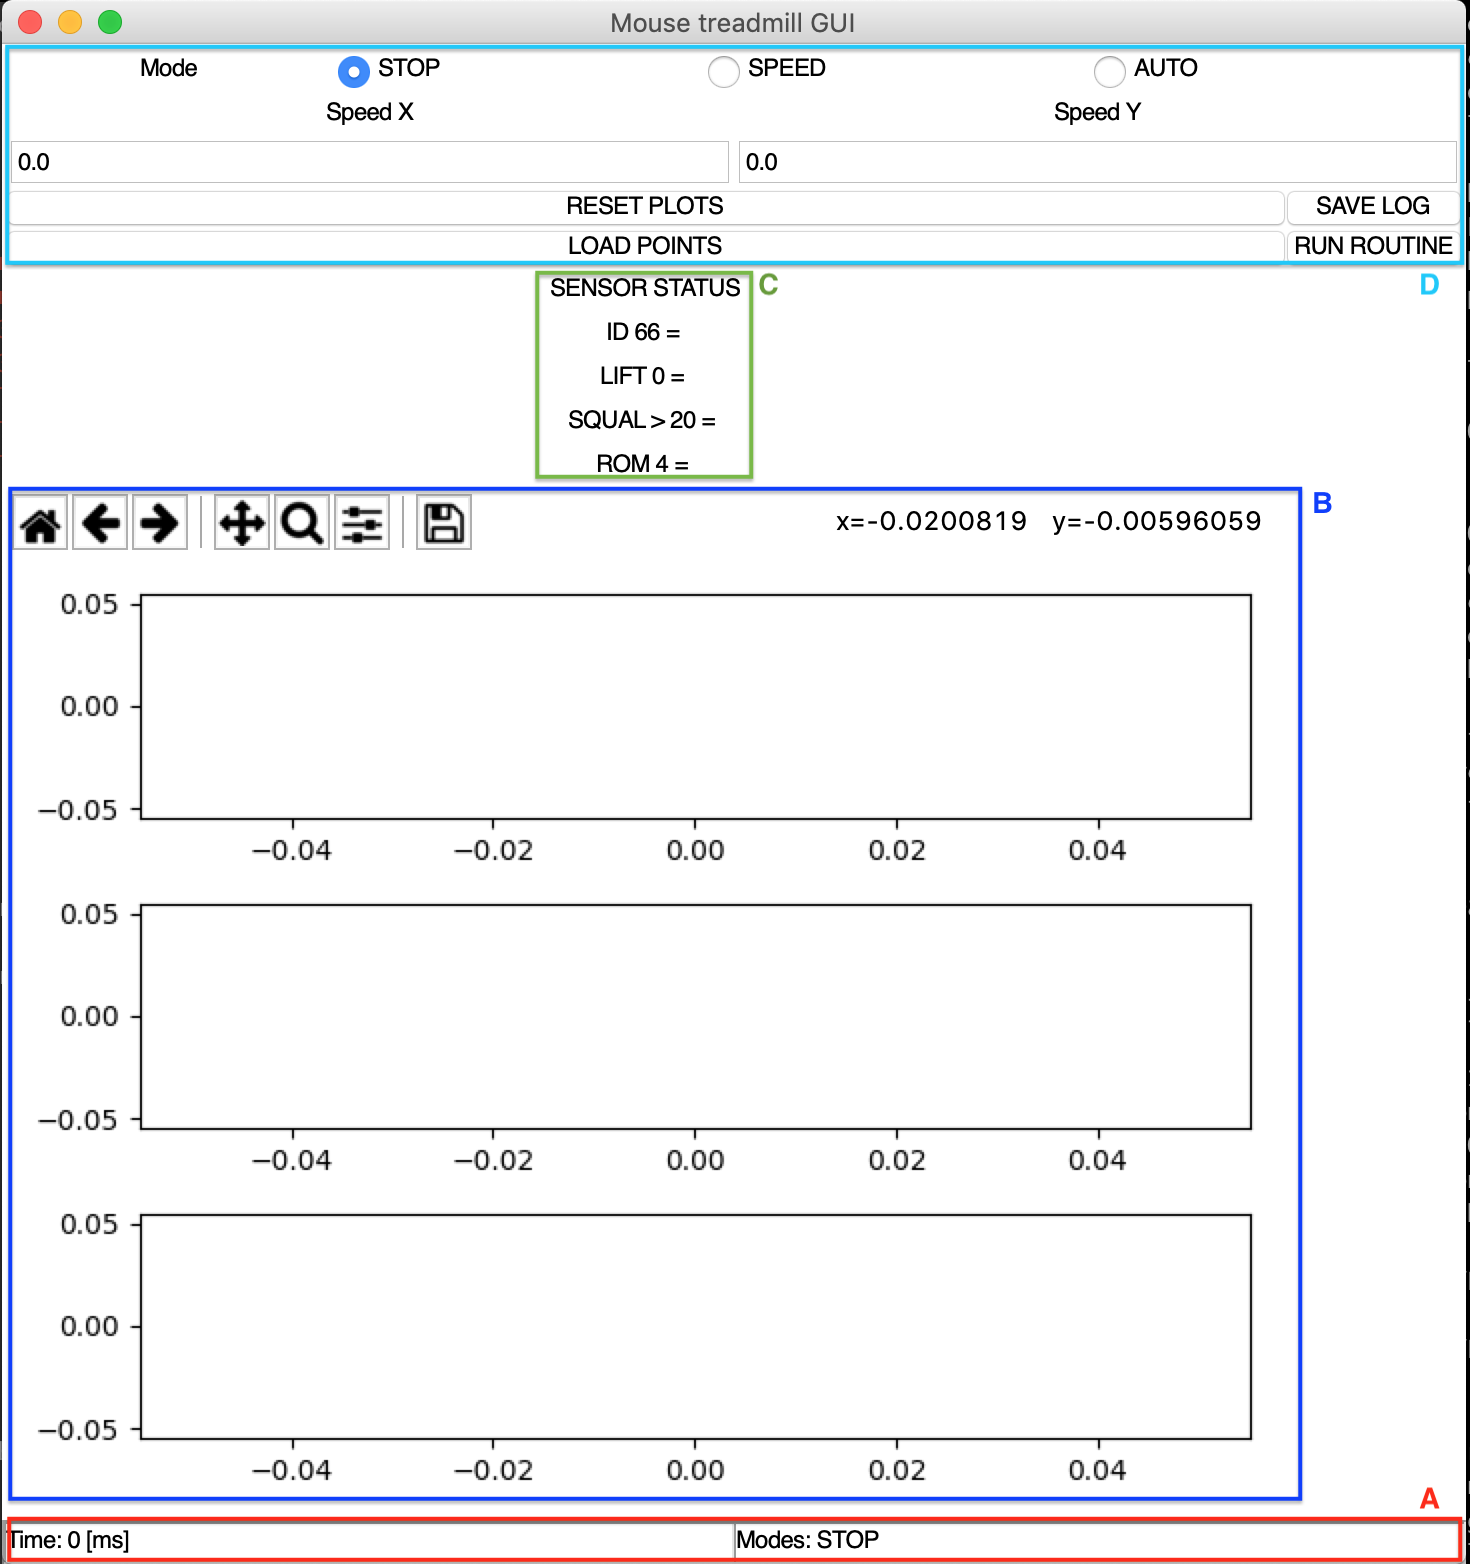
\includegraphics[width=1\linewidth]{fig/GUI.png}
	\caption{GUI screenshot on a MAC.}\label{fig:GUI}
\end{figure}
Figure \ref{fig:GUI} is taken on a MAC, the GUI have the same functionalities on other platforms, but it might look different. The library used to design the GUI is Appjar, which is compatible with MAC, LINUX and Windows.
\begin{itemize}
	\item \textcolor{red}{\textbf{A}} In this region the content of the HEARTBEAT message are presented. Time is the time from boot of the system in milliseconds. Modes is the mode in which the stm32 is. The mode can be STOP, SPEED AUTO or RUNNING.
	\item \textcolor{blue}{\textbf{B}} In this region the real-time data are plotted. The top plot shows the X and Y motor signals, the middle one shows the X and Y speed setpoints and the bottom one shows the motor signal. By using the top left buttons it is possible to save the plots and navigate them, it is advisable to store the data and plot them afterwards using another script for better analysis due to the fast update of the plots.
	\item \textcolor{green}{\textbf{C}} In this region data from the sensors are displayed. ID is the product ID of the sensor and is used to verify that the communication between the sensor and the board is working correctly. LIFT is 0 if the sensor detects correctly the surface and 1 if it does not. SQUAL is the surface quality information. This value should be greater than 20 for the measure to be good. ROM is the SROM ID of the sensor. This value is used to verify that the SROM is flashed correctly during initialization. If everything is working correctly you should see something like table \ref{tab:sens_corr}
	\begin{table}[H]
		\centering
		\begin{tabular}{|c|} 
			\hline
			SENSOR STATUS\\ 
			ID 66 = 66 | 66\\
			LIFT 0 = 0 | 0\\
			SQUAL > 20 = 34 | 43\\
			ROM 4 = 4 | 4\\
			\hline
		\end{tabular} 
		\caption{Example of GUI output for sensor initialized and connected correctly and detecting a good quality surface. Before = the name of the information and its correct value are shown, after the sensor x | sensor y readings are displayed.}
		\label{tab:sens_corr}
	\end{table}
	\item \textcolor{cyan}{\textbf{D}} 
	In this region the input from the user are taken. In the first line the user can select the mode to be used:
	\begin{itemize}
		\item \textbf{STOP}: When this mode is selected the motor are stopped.
		\item \textbf{SPEED}: When this mode is selected the motor setpoints can be typed in the two entries under the Speed X and Speed Y labels.
		\item \textbf{AUTO}: When this mode is selected the user can load the points of the routine on the board (Modes: LOAD) and then run the routine (Modes: RUNNING).
	\end{itemize} 
	Finally the RESET PLOTS button is used to reset the plot in case of reset on the board, the SAVE LOG button stores all the data received in a file in /log/log.txt. This file is overwritten every time so if you need the data please copy them in a safe place. The LOAD POINTS sends the points defined in routine.py to the board. This will work only if the mode is set to AUTO (should see LOAD in Modes in  \textcolor{red}{\textbf{A}} and the time should not be updated). Finally the RUN ROUTINE button starts the routine on the board (the board goes in mode RUNNING).	
\end{itemize}  
\begin{figure}[H]
	\centering
	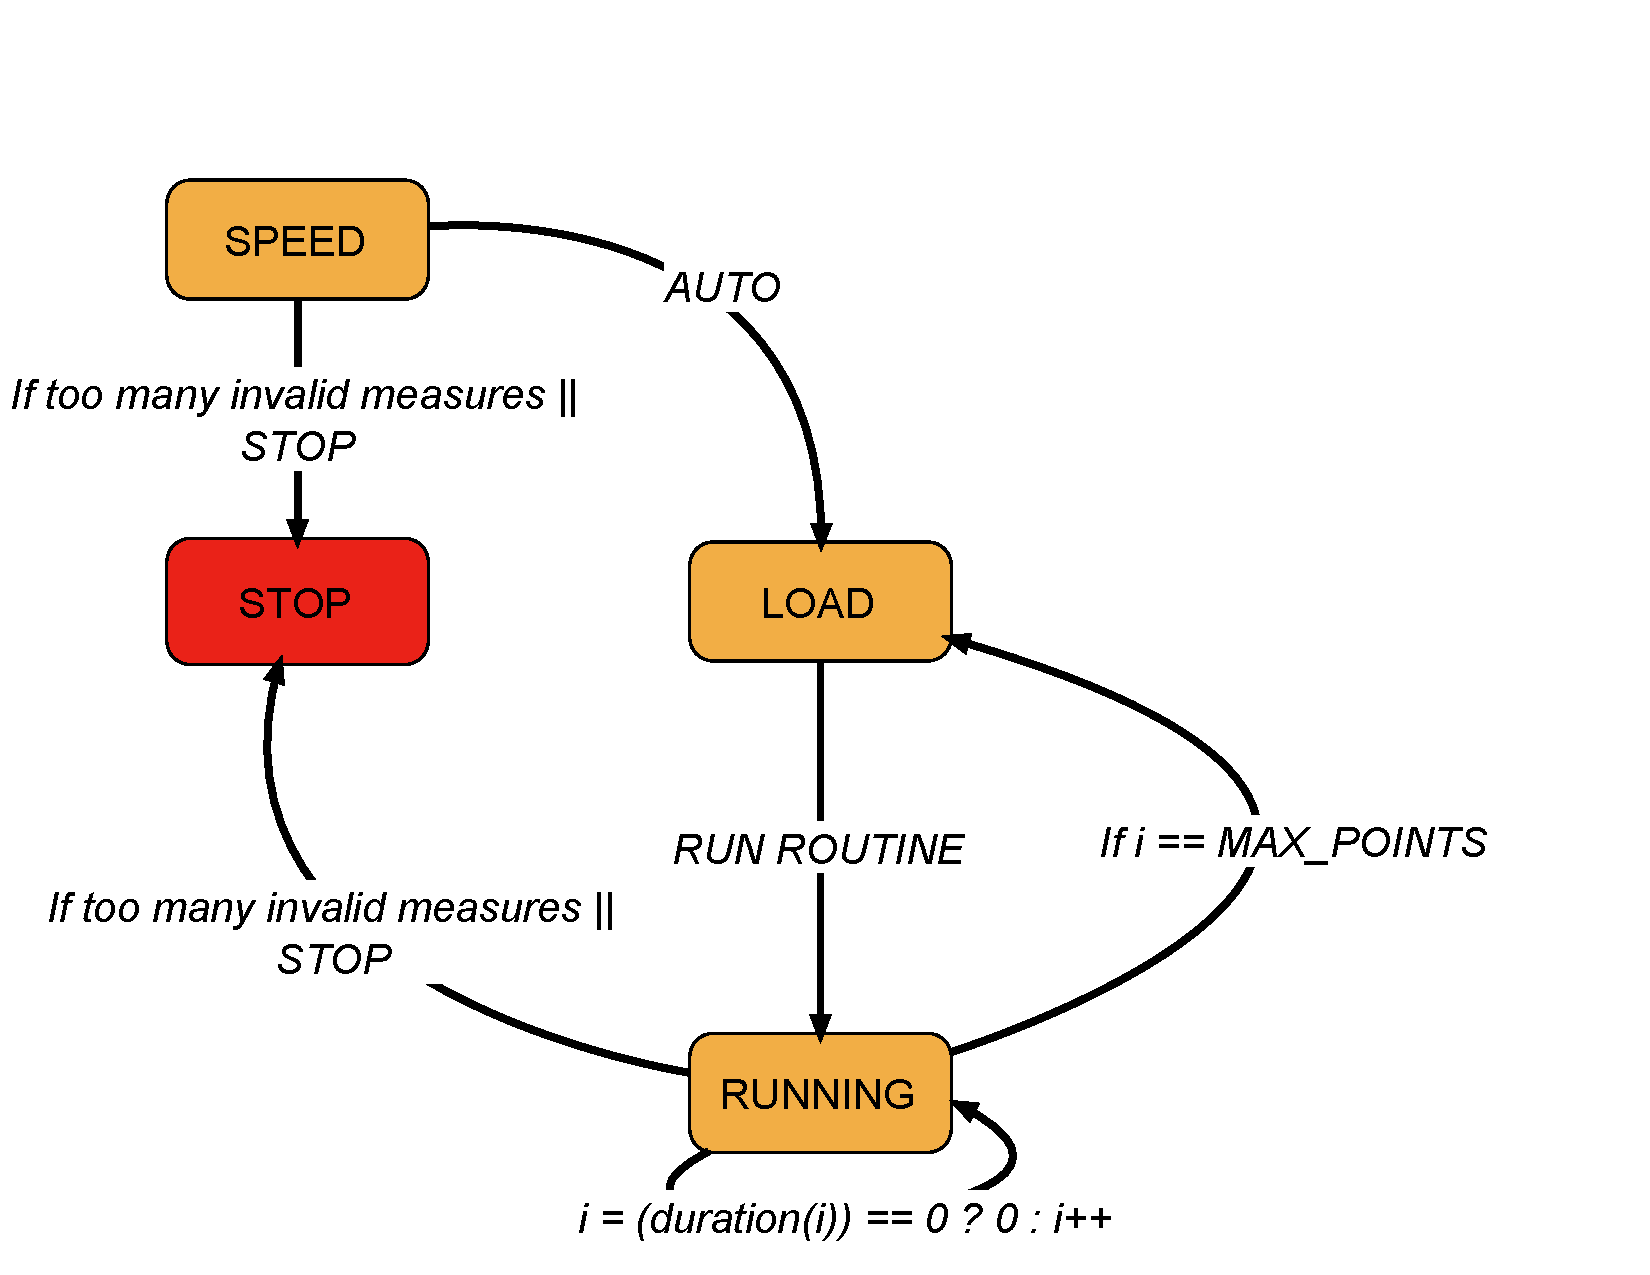
\includegraphics[width=0.7\linewidth]{fig/FSM.pdf}
	\caption{Finite state machine of the mouse treadmill.}\label{fig:FSM}
\end{figure}
The finite state machine of the machine is shown in figure \ref{fig:FSM}. All the capital letters conditions (except for MAX\_POINTS) are widgets on the GUI that can be pressed by the user while using the machine.
\subsection{How to write a routine}
In this section the way to properly define a routine is described. 
An example routine is provided in MouseTreadmillPC/python/routine.py. The routine is a python dictionary containing a list of durations, setpoint\_x and setpoint\_y. The two setpoints define the desired speed along x and y, while the duration is the time span during which the two setpoints are applied. One should notice that the system time is discrete and increased every millisecond, moreover one should take into account the settling time for the control and the maximum acceleration provided by the motors to do a proper discretization of the desired speed profile.\\
A duration of 0 means that the end of the routine is reached and the routine is started again at the first point defined. A maximum of 255 points can be defined, if more points are needed the id of the point have to be changed from type uint8\_t to uint16\_t to allow for IDs above 255. A memory limitation is still present, but for a number of points above 1'000.
\subsection{How to extend the system}
To extend the system with new messages and features the main operation consist in modifying \ref{app:mavlink}. This files describes all the messages and constants used in the communication protocol, thus it possible to add/modify them. If you need to create a new message or constant, please have a look at the already defined ones and use them as a template. 
To extend the system please follow the following steps:
\begin{enumerate}
	\item Get the basic system installed correctly, for that see \ref{sec:install}.
	\item Modify \ref{app:mavlink} (mouse.xml) as needed.
	\item Generate the C libraries for the STM32, for that you need:
	\begin{lstlisting}[style = Bashstyle]
	$ cd 3DMouseTreadmill/mavlink
	$ python 3 mavgenerate.py
	\end{lstlisting}
	Now a GUI asking you information appear, this must be filled as follow:
	\begin{itemize}
		\item \textbf{XML} there you indicate the mouse.xml file that was previously modified
		\item \textbf{Out} there you indicate the 3DMouseTreadmill/MAVLink Library/
		\item \textbf{Language} Choose C
		\item \textbf{Protocol} Choose 2.0
		\item \textbf{Validate} Choose Yes
		\item \textbf{Validate Units} Choose Yes
	\end{itemize}
	Now you can press on generate.
	The GUI should be similar to figure \ref{fig:gen_c}.
	If some errors are shown, correct them and try again.
	\item Adapt the code in the STM32 project if needed.
	\item Generate the python libraries for the PC, for that you need:
	\begin{enumerate}
		\item Run mavgenerate.py (if not still running)
		\begin{lstlisting}[style = Bashstyle]
		$ python 3 mavgenerate.py
		\end{lstlisting}
		Now a GUI asking you information appear, this must be filled as follow:
		\begin{itemize}
			\item \textbf{XML} there you indicate the mouse.xml file that was previously modified
			\item \textbf{Out} there you indicate the 3DMouseTreadmill/mouse.py
			\item \textbf{Language} Choose Python
			\item \textbf{Protocol} Choose 2.0
			\item \textbf{Validate} Choose Yes
			\item \textbf{Validate Units} Choose Yes
		\end{itemize}
		Now you can press on generate.
		The GUI should be similar to figure \ref{fig:gen_py}.
		If some errors are shown, correct them and try again.
		\item Change directory to the parent one
		\begin{lstlisting}[style = Bashstyle]
		$ cd ../
		\end{lstlisting}
		\item repeat the installation guide (see \ref{sec:install}) from point 3. 
	\end{enumerate}
	\item Adapt the python code if necessary. 	
\end{enumerate}
\begin{figure}[H]
	\centering
	\begin{subfigure}[b]{0.4\textwidth}
		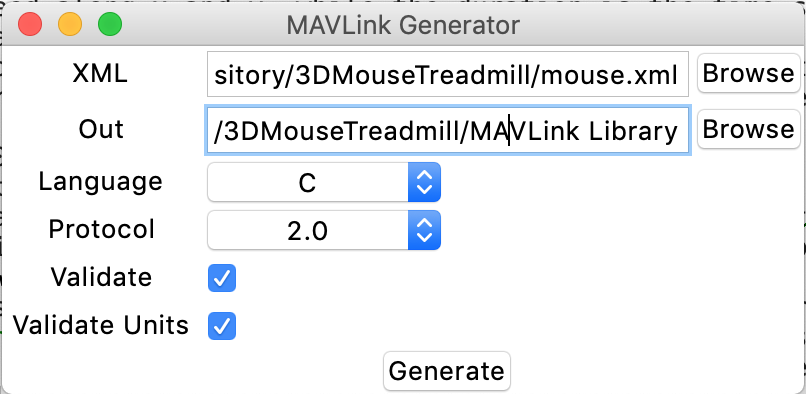
\includegraphics[width=\textwidth]{fig/gen_c}
		\caption{C libraries.}
		\label{fig:gen_c}
	\end{subfigure}
	\begin{subfigure}[b]{0.4\textwidth}
		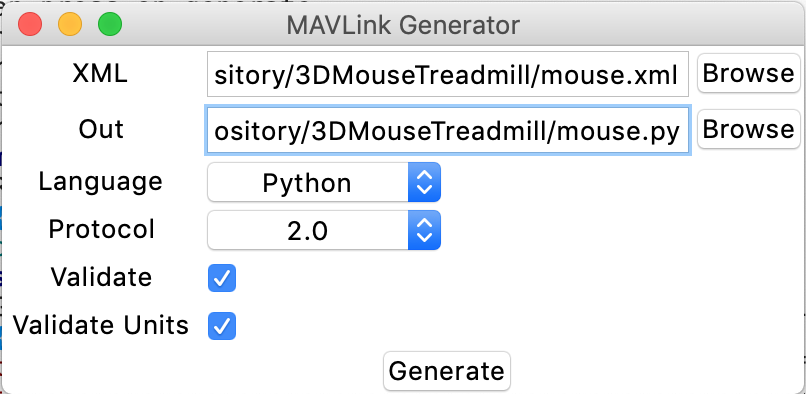
\includegraphics[width=\textwidth]{fig/gen_py}
		\caption{python libraries.}
		\label{fig:gen_py}
	\end{subfigure}
	\caption{mavgenerate GUI screenshots properly setup for generating python and C libraries.}
\end{figure}

\newpage
\lhead{ }
\begin{thebibliography}{100}
	
	\bibitem{Ole}Jared M. Cregg, Roberto Leiras, Alexia Montalant, Ian R. Wickersham, and Ole Kiehn, \textit{Brainstem Neurons that Command Left/Right Locomotor Asymmetries} 
	\bibitem{mavlink} MAVLink Developer Guide, \textit{https://mavlink.io/en/}
	\bibitem{py} Python website, \textit{https://www.python.org/downloads/}
	
	\bibitem{sar} Robin R. Murphy, Eric Steimle et al. \textit{Cooperative Use of Unmanned Sea Surface and Micro Aerial Vehicles at Hurricane Wilma},Journal of Field Robotics,2008
	\bibitem{eco}     Kenzo Nonami, Farid Kendoul, Satoshi Suzuki, Wei Wang, Daisuke Nakazawa,\textit{Autonomous Flying Robots}, Springer, 2010.
	\bibitem{roll} G. Sachs, \textit{What Can Be Learned from Unique Lateral-Directional Dynamics Properties of Birds for Mini-Aircraft}, Atmospheric Flight Mechanics Conference and Exhibit, 2007
	%\bibitem{ref1} Onur Bilgen, Kevin B. Kochersberger, and Daniel J. Inman, \textit{Novel, Bidirectional, Variable-Camber Airfoil via Macro-Fiber Composite Actuators}, Journal of aircraft Vol. 47, No. 1, January–February 2010.
	\bibitem{real_plane} R. Pecora, F. Amoroso, and L. Lecce, \textit{Effectiveness of Wing Twist Morphing in Roll Control}, Journal of aircraft Vol. 49, No. 6, November–December 2012
	\bibitem{ref3} Osgar John Ohanian III, Christopher Hickling, Brandon Stiltner, Etan D. Karni, \textit{Piezoelectric Morphing versus Servo-Actuated MAV Control Surfaces}, 53rd AIAA/ASME/ASCE/AHS/ASC Structures, Structural Dynamics and Materials Conference, 2012
	\bibitem{ref4} Helen M. Garcia , Mujahid Abdulrahim and Rick Lind, \textit{Roll control for a micro air vehicle using active wing morphing}, AIAA Guidance, Navigation, and Control Conference and Exhibit, 2003
	\bibitem{ref5} Mujahid Abdulrahim, Helen Garcia, and Rick Lind, \textit{Flight Characteristics of Shaping the Membrane Wing of a Micro Air Vehicle}, Journal of aircraft Vol. 42, No. 1, January–February 2005
	\bibitem{ref6} M. Di Luca, S. Mintchev, G. Heitz, F. Noca and D. Floreano, \textit{Bioinspired morphing wings for extended flight envelope and roll control of small drones}, Interface Focus 7, 2017
	\bibitem{urb_env} William E. Green and Paul Y. Oh, \textit{A Hybrid MAV for Ingress and Egress of Urban Environments}, IEEE transactions on robotics, 2009
	\bibitem{twist} Bret Stanford, Mujahid Abdulrahim, Rick Lind, and Peter Ifju, \textit{Actuation for Roll Control of a Micro Air Vehicle}, Journal of aircraft,  2007
	\bibitem{rev} Juan Carlos Gomez and Ephrahim Garcia, \textit{Morphing unmanned aerial vehicles}, Smart materials and structures, 2011.
	\bibitem{book} E.L. Houghton, P.W. Carpenter, Steven H. Collicott and Daniel T. Valentine, \textit{Aerodynamics for engineering students}, Seventh edition.
	\bibitem{fire} Pero Skorput, Sadko Mandzuka, Hrvoje Vojvodic, \textit{The Use of Unmanned Aerial Vehicles for Forest Fire Monitoring }, 58th International Symposium ELMAR, 2016
	\bibitem{city} David Gallacher, \textit{Drone Applications for Environmental Management in Urban Spaces: A Review}, International Journal of Sustainable Land Use and Urban Planning, 2016
	\bibitem{disaster} Ludovic Apvrille, Tullio Tanzi, and Jean-Luc Dugelay \textit{Autonomous Drones for Assisting Rescue Services within the context of Natural Disasters}, XXXIth URSI General Assembly and Scientific Symposium, 2014
\end{thebibliography}
\bibliographystyle{plainnat}
\listoffigures
\listoftables
\appendix
\section{MAVLink dialect description file}\label{app:mavlink}
\lstinputlisting[language=XML]{../mouse.xml}
\section{Code for STM32 NUCLEO 64 board}
\subsection{Main}
\lstinputlisting[style=CStyle]{../MouseTreadmillSTM32Project/Core/Inc/main.h}
\lstinputlisting[style=CStyle]{../MouseTreadmillSTM32Project/Core/Src/main.c}
\subsection{Treadmill driver}
\lstinputlisting[style=CStyle]{../CodeSTM32/src/mouseDriver.c}
\lstinputlisting[style=CStyle]{../CodeSTM32/src/mouseDriver.h}
\subsection{Sensor driver}
\lstinputlisting[style=CStyle]{../CodeSTM32/src/sensorDriver.c}
\lstinputlisting[style=CStyle]{../CodeSTM32/src/sensorDriver.h}
\subsection{Code for unit tests}
\lstinputlisting[style=CStyle]{../CodeSTM32/test/display.h}
\lstinputlisting[style=CStyle]{../CodeSTM32/test/main.c}
\lstinputlisting[style=CStyle]{../CodeSTM32/test/mock_mouseDriver.h}
\lstinputlisting[style=CStyle]{../CodeSTM32/test/mock_sensorDriver.h}
\lstinputlisting[style=CStyle]{../CodeSTM32/test/test_mouseDriver.h}
\lstinputlisting[style=CStyle]{../CodeSTM32/test/test_sensorDriver.h}
\lstinputlisting[style=CStyle]{../CodeSTM32/test/test_mouseDriver.c}
\lstinputlisting[style=CStyle]{../CodeSTM32/test/test_sensorDriver.c}
\subsection{Build script}
\lstinputlisting[style=CStyle]{../CodeSTM32/src/build.sh}

\section{Code for PC}
\subsection{GUI}
\lstinputlisting[style=PyStyle]{../MouseTreadmillPC/python/mouseController.py}
\subsection{Routine example}
\lstinputlisting[style=PyStyle]{../MouseTreadmillPC/python/routine.py}
\section{Data-sheets}
\subsection{Sensor Data-sheet }\label{app:PMW3660}
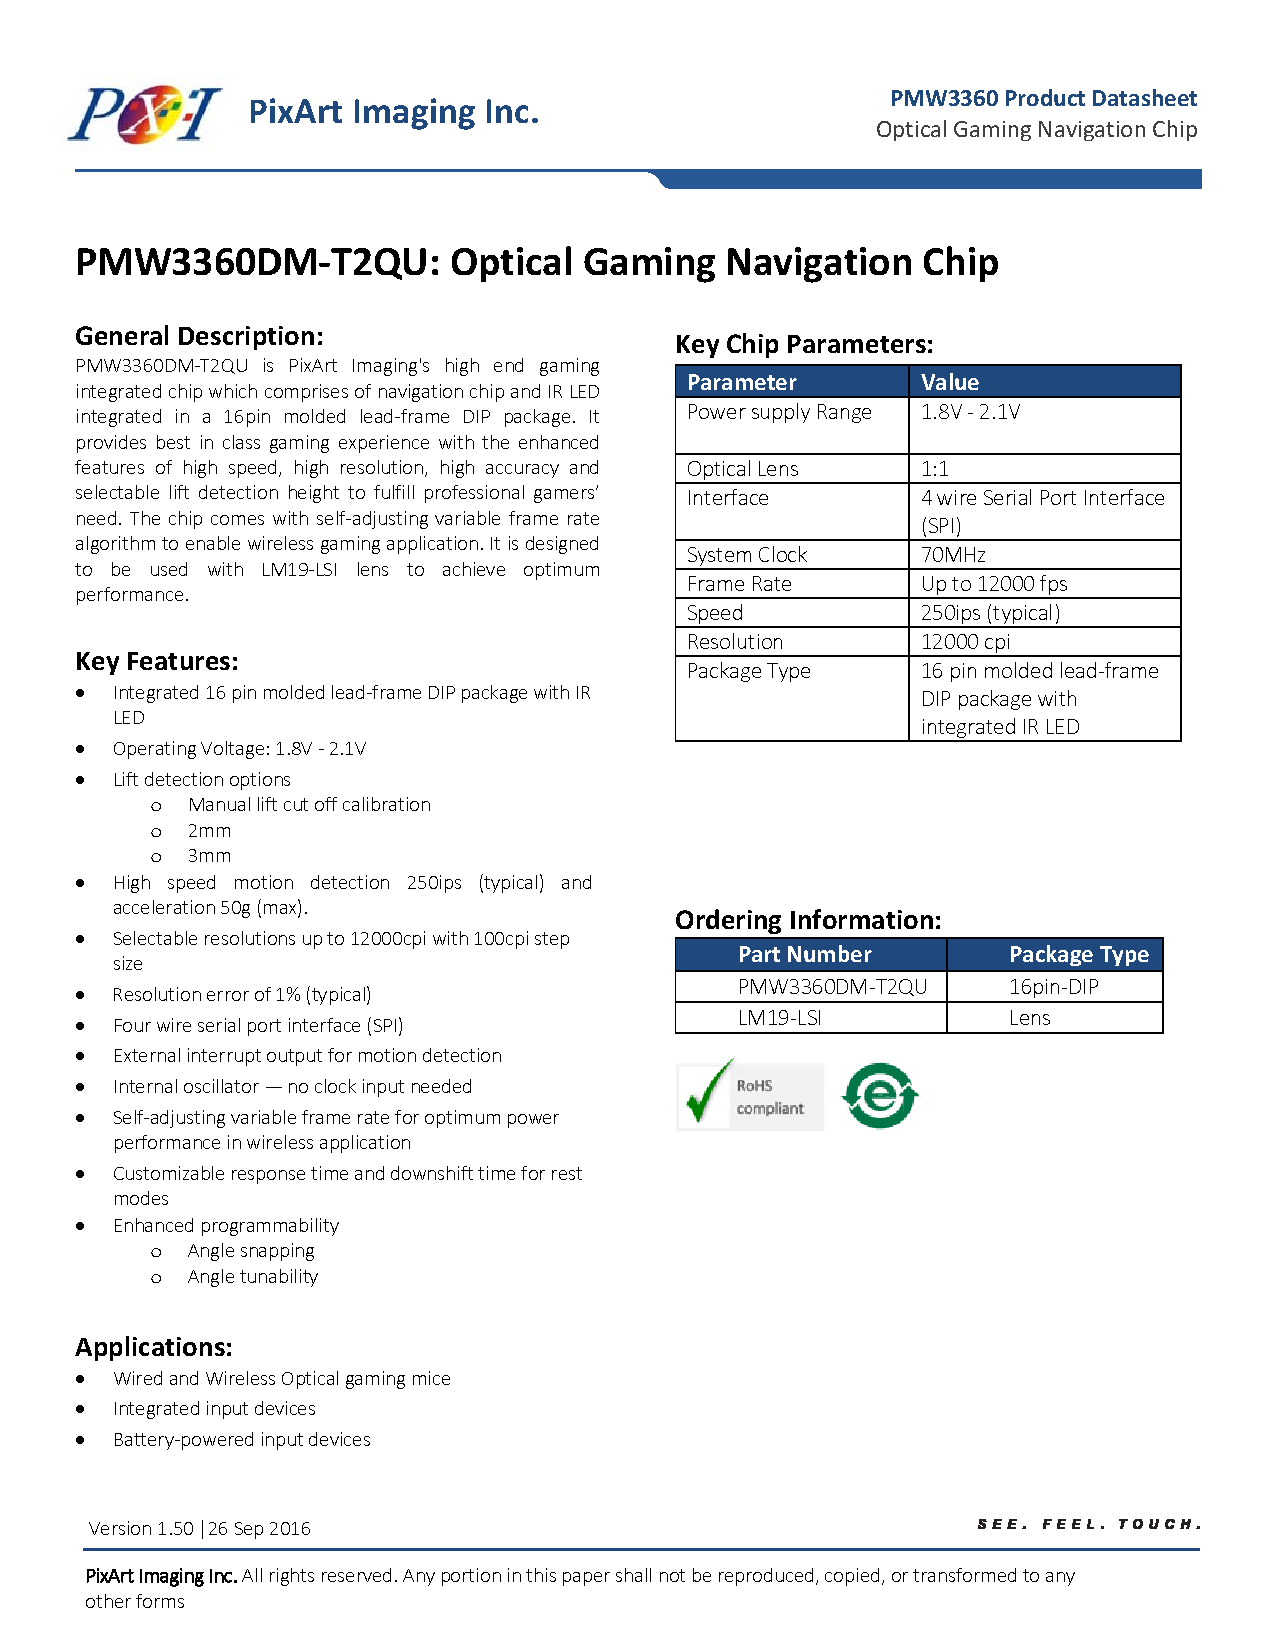
\includepdf[pages=-]{../resources/sensorDatasheet.pdf}
%\let\mypdfximage\pdfximage\def\pdfximage{\immediate\mypdfximage}\documentclass[twoside]{book}

%% moved from doxygen.sty due to workaround for LaTex 2019 version and unmaintained tabu package
\usepackage{ifthen}
\ifx\requestedLaTeXdate\undefined
\usepackage{array}
\else
\usepackage{array}[=2016-10-06]
\fi
%%
% Packages required by doxygen
\usepackage{fixltx2e}
\usepackage{calc}
\usepackage{doxygen}
\usepackage{graphicx}
\usepackage[utf8]{inputenc}
\usepackage{makeidx}
\usepackage{multicol}
\usepackage{multirow}
\PassOptionsToPackage{warn}{textcomp}
\usepackage{textcomp}
\usepackage[nointegrals]{wasysym}
\usepackage[table]{xcolor}
\usepackage{ifpdf,ifxetex}

% Font selection
\usepackage[T1]{fontenc}
\usepackage[scaled=.90]{helvet}
\usepackage{courier}
\usepackage{amssymb}
\usepackage{sectsty}
\renewcommand{\familydefault}{\sfdefault}
\allsectionsfont{%
  \fontseries{bc}\selectfont%
  \color{darkgray}%
}
\renewcommand{\DoxyLabelFont}{%
  \fontseries{bc}\selectfont%
  \color{darkgray}%
}
\newcommand{\+}{\discretionary{\mbox{\scriptsize$\hookleftarrow$}}{}{}}

% Arguments of doxygenemoji:
% 1) ':<text>:' form of the emoji, already "LaTeX"-escaped
% 2) file with the name of the emoji without the .png extension
% in case image exist use this otherwise use the ':<text>:' form
\newcommand{\doxygenemoji}[2]{%
  \IfFileExists{./#2.png}{\raisebox{-0.1em}{\includegraphics[height=0.9em]{./#2.png}}}{#1}%
}
% Page & text layout
\usepackage{geometry}
\geometry{%
  a4paper,%
  top=2.5cm,%
  bottom=2.5cm,%
  left=2.5cm,%
  right=2.5cm%
}
\tolerance=750
\hfuzz=15pt
\hbadness=750
\setlength{\emergencystretch}{15pt}
\setlength{\parindent}{0cm}
\newcommand{\doxynormalparskip}{\setlength{\parskip}{3ex plus 2ex minus 2ex}}
\newcommand{\doxytocparskip}{\setlength{\parskip}{1ex plus 0ex minus 0ex}}
\doxynormalparskip
\makeatletter
\renewcommand{\paragraph}{%
  \@startsection{paragraph}{4}{0ex}{-1.0ex}{1.0ex}{%
    \normalfont\normalsize\bfseries\SS@parafont%
  }%
}
\renewcommand{\subparagraph}{%
  \@startsection{subparagraph}{5}{0ex}{-1.0ex}{1.0ex}{%
    \normalfont\normalsize\bfseries\SS@subparafont%
  }%
}
\makeatother

% Headers & footers
\usepackage{fancyhdr}
\pagestyle{fancyplain}
\fancyhead[LE]{\fancyplain{}{\bfseries\thepage}}
\fancyhead[CE]{\fancyplain{}{}}
\fancyhead[RE]{\fancyplain{}{\bfseries\leftmark}}
\fancyhead[LO]{\fancyplain{}{\bfseries\rightmark}}
\fancyhead[CO]{\fancyplain{}{}}
\fancyhead[RO]{\fancyplain{}{\bfseries\thepage}}
\fancyfoot[LE]{\fancyplain{}{}}
\fancyfoot[CE]{\fancyplain{}{}}
\fancyfoot[RE]{\fancyplain{}{\bfseries\scriptsize Generated by Doxygen }}
\fancyfoot[LO]{\fancyplain{}{\bfseries\scriptsize Generated by Doxygen }}
\fancyfoot[CO]{\fancyplain{}{}}
\fancyfoot[RO]{\fancyplain{}{}}
\renewcommand{\footrulewidth}{0.4pt}
\renewcommand{\chaptermark}[1]{%
  \markboth{#1}{}%
}
\renewcommand{\sectionmark}[1]{%
  \markright{\thesection\ #1}%
}

% Indices & bibliography
\usepackage{natbib}
\usepackage[titles]{tocloft}
\setcounter{tocdepth}{3}
\setcounter{secnumdepth}{5}
\makeindex

\usepackage{newunicodechar}
  \newunicodechar{⁻}{${}^{-}$}% Superscript minus
  \newunicodechar{²}{${}^{2}$}% Superscript two
  \newunicodechar{³}{${}^{3}$}% Superscript three

% Hyperlinks (required, but should be loaded last)
\ifpdf
  \usepackage[pdftex,pagebackref=true]{hyperref}
\else
  \ifxetex
    \usepackage[pagebackref=true]{hyperref}
  \else
    \usepackage[ps2pdf,pagebackref=true]{hyperref}
  \fi
\fi

\hypersetup{%
  colorlinks=true,%
  linkcolor=blue,%
  citecolor=blue,%
  unicode%
}

% Custom commands
\newcommand{\clearemptydoublepage}{%
  \newpage{\pagestyle{empty}\cleardoublepage}%
}

\usepackage{caption}
\captionsetup{labelsep=space,justification=centering,font={bf},singlelinecheck=off,skip=4pt,position=top}

\usepackage{etoc}
\etocsettocstyle{\doxytocparskip}{\doxynormalparskip}
\renewcommand{\numberline}[1]{#1~}
%===== C O N T E N T S =====

\begin{document}

% Titlepage & ToC
\hypersetup{pageanchor=false,
             bookmarksnumbered=true,
             pdfencoding=unicode
            }
\pagenumbering{alph}
\begin{titlepage}
\vspace*{7cm}
\begin{center}%
{\Large 3D\+Mouse\+Treadmill \\[1ex]\large 0 }\\
\vspace*{1cm}
{\large Generated by Doxygen 1.8.16}\\
\end{center}
\end{titlepage}
\clearemptydoublepage
\pagenumbering{roman}
\tableofcontents
\clearemptydoublepage
\pagenumbering{arabic}
\hypersetup{pageanchor=true}

%--- Begin generated contents ---
\chapter{File Index}
\doxysection{File List}
Here is a list of all files with brief descriptions\+:\begin{DoxyCompactList}
\item\contentsline{section}{Code S\+T\+M32/\mbox{\hyperlink{mouse_driver_8c}{mouse\+Driver.\+c}} \\*Implementation of the driver for the mouse treadmil project }{\pageref{mouse_driver_8c}}{}
\item\contentsline{section}{Code S\+T\+M32/\mbox{\hyperlink{mouse_driver_8h}{mouse\+Driver.\+h}} \\*Header of the driver for the mouse treadmil project }{\pageref{mouse_driver_8h}}{}
\item\contentsline{section}{Code S\+T\+M32/\mbox{\hyperlink{utils_8h}{utils.\+h}} }{\pageref{utils_8h}}{}
\end{DoxyCompactList}

\chapter{File Documentation}
\hypertarget{mouse_driver_8c}{}\doxysection{Code S\+T\+M32/mouse\+Driver.c File Reference}
\label{mouse_driver_8c}\index{Code STM32/mouseDriver.c@{Code STM32/mouseDriver.c}}


Implementation of the driver for the mouse treadmil project.  


{\ttfamily \#include \char`\"{}mouse\+Driver.\+h\char`\"{}}\newline
\doxysubsection*{Functions}
\begin{DoxyCompactItemize}
\item 
void \mbox{\hyperlink{mouse_driver_8c_a78891a5c0a9ff59e8de3479cef3dd708}{mouse\+Driver\+\_\+init\+Setpoint}} (void)
\item 
void \mbox{\hyperlink{mouse_driver_8c_a399080e7e42aa3cf13e3ae5c6012b731}{mouse\+Driver\+\_\+init\+Time}} (void)
\item 
void \mbox{\hyperlink{mouse_driver_8c_ae21a55ca0039131ed41b563efbb81ddb}{mouse\+Driver\+\_\+init\+Mode}} (void)
\item 
void \mbox{\hyperlink{mouse_driver_8c_ad79b2fdfdd673bb416b89de2bd80927d}{mouse\+Driver\+\_\+get\+Speed\+From\+Sensors}} (void)
\item 
void \mbox{\hyperlink{mouse_driver_8c_aa5609bff60e6d530873ab05bb4dc8e97}{mouse\+Driver\+\_\+set\+Setpoint}} (const mavlink\+\_\+speed\+\_\+setpoint\+\_\+t speed)
\item 
void \mbox{\hyperlink{mouse_driver_8c_a237f0960175af336ca81667d7eb9ef2e}{mouse\+Driver\+\_\+set\+Mode}} (uint8\+\_\+t mode)
\item 
void \mbox{\hyperlink{mouse_driver_8c_a0c549479547ef441f7424ffcbe47de95}{mouse\+Driver\+\_\+send\+Msg}} (uint32\+\_\+t msgid)
\item 
void \mbox{\hyperlink{mouse_driver_8c_a1b501a2d737cbe2636dc76e7d7c9378e}{mouse\+Driver\+\_\+init}} (void)
\begin{DoxyCompactList}\small\item\em Function for initializing the mouse\+Driver. \end{DoxyCompactList}\item 
void \mbox{\hyperlink{mouse_driver_8c_aa7d22c0c2f293182c6197e25e5afb352}{mouse\+Driver\+\_\+set\+Time}} (const uint32\+\_\+t time)
\item 
uint32\+\_\+t \mbox{\hyperlink{mouse_driver_8c_a7908648bbda149bdf1ef821097039684}{mouse\+Driver\+\_\+get\+Time}} (void)
\item 
void \mbox{\hyperlink{mouse_driver_8c_ac6ff4f7ea298a0b01815904468bb29da}{mouse\+Driver\+\_\+read\+Msg}} (const mavlink\+\_\+message\+\_\+t msg)
\item 
void \mbox{\hyperlink{mouse_driver_8c_aaeee34eedb0741b6360ad62ac296cc7e}{mouse\+Driver\+\_\+idle}} (void)
\item 
void \mbox{\hyperlink{mouse_driver_8c_ae148c84e3642827c8d5c34a675d65739}{mouse\+Driver\+\_\+control\+I\+SR}} (void)
\end{DoxyCompactItemize}
\doxysubsection*{Variables}
\begin{DoxyCompactItemize}
\item 
static uint32\+\_\+t \mbox{\hyperlink{mouse_driver_8c_a8e8611558b7ab767b1685a6a350aee53}{actual\+\_\+time}} = 0
\begin{DoxyCompactList}\small\item\em Global variable for time keeping. \end{DoxyCompactList}\item 
static uint8\+\_\+t \mbox{\hyperlink{mouse_driver_8c_a7e2c75a51747c0c5f00ad6c672bc3024}{actual\+\_\+mode}} = M\+O\+U\+S\+E\+\_\+\+M\+O\+D\+E\+\_\+\+S\+T\+OP
\item 
static mavlink\+\_\+speed\+\_\+info\+\_\+t \mbox{\hyperlink{mouse_driver_8c_aa5490b06dbe7d61f3661c8afbd10d317}{actual\+\_\+speed\+\_\+measure}}
\item 
static mavlink\+\_\+speed\+\_\+setpoint\+\_\+t \mbox{\hyperlink{mouse_driver_8c_a2ed2ab5427f1ccd8753023817343ac75}{actual\+\_\+speed\+\_\+setpoint}}
\item 
static mavlink\+\_\+motor\+\_\+setpoint\+\_\+t \mbox{\hyperlink{mouse_driver_8c_ad6abb9303429a23fb0456e5b155cc37c}{actual\+\_\+motor\+\_\+signal}}
\end{DoxyCompactItemize}


\doxysubsection{Detailed Description}
Implementation of the driver for the mouse treadmil project. 

\begin{DoxyAuthor}{Author}
Didier Negretto 
\end{DoxyAuthor}


\doxysubsection{Function Documentation}
\mbox{\Hypertarget{mouse_driver_8c_ae148c84e3642827c8d5c34a675d65739}\label{mouse_driver_8c_ae148c84e3642827c8d5c34a675d65739}} 
\index{mouseDriver.c@{mouseDriver.c}!mouseDriver\_controlISR@{mouseDriver\_controlISR}}
\index{mouseDriver\_controlISR@{mouseDriver\_controlISR}!mouseDriver.c@{mouseDriver.c}}
\doxysubsubsection{\texorpdfstring{mouseDriver\_controlISR()}{mouseDriver\_controlISR()}}
{\footnotesize\ttfamily void mouse\+Driver\+\_\+control\+I\+SR (\begin{DoxyParamCaption}\item[{void}]{ }\end{DoxyParamCaption})}

\mbox{\Hypertarget{mouse_driver_8c_ad79b2fdfdd673bb416b89de2bd80927d}\label{mouse_driver_8c_ad79b2fdfdd673bb416b89de2bd80927d}} 
\index{mouseDriver.c@{mouseDriver.c}!mouseDriver\_getSpeedFromSensors@{mouseDriver\_getSpeedFromSensors}}
\index{mouseDriver\_getSpeedFromSensors@{mouseDriver\_getSpeedFromSensors}!mouseDriver.c@{mouseDriver.c}}
\doxysubsubsection{\texorpdfstring{mouseDriver\_getSpeedFromSensors()}{mouseDriver\_getSpeedFromSensors()}}
{\footnotesize\ttfamily void mouse\+Driver\+\_\+get\+Speed\+From\+Sensors (\begin{DoxyParamCaption}\item[{void}]{ }\end{DoxyParamCaption})}

\mbox{\Hypertarget{mouse_driver_8c_a7908648bbda149bdf1ef821097039684}\label{mouse_driver_8c_a7908648bbda149bdf1ef821097039684}} 
\index{mouseDriver.c@{mouseDriver.c}!mouseDriver\_getTime@{mouseDriver\_getTime}}
\index{mouseDriver\_getTime@{mouseDriver\_getTime}!mouseDriver.c@{mouseDriver.c}}
\doxysubsubsection{\texorpdfstring{mouseDriver\_getTime()}{mouseDriver\_getTime()}}
{\footnotesize\ttfamily uint32\+\_\+t mouse\+Driver\+\_\+get\+Time (\begin{DoxyParamCaption}\item[{void}]{ }\end{DoxyParamCaption})}

\mbox{\Hypertarget{mouse_driver_8c_aaeee34eedb0741b6360ad62ac296cc7e}\label{mouse_driver_8c_aaeee34eedb0741b6360ad62ac296cc7e}} 
\index{mouseDriver.c@{mouseDriver.c}!mouseDriver\_idle@{mouseDriver\_idle}}
\index{mouseDriver\_idle@{mouseDriver\_idle}!mouseDriver.c@{mouseDriver.c}}
\doxysubsubsection{\texorpdfstring{mouseDriver\_idle()}{mouseDriver\_idle()}}
{\footnotesize\ttfamily void mouse\+Driver\+\_\+idle (\begin{DoxyParamCaption}\item[{void}]{ }\end{DoxyParamCaption})}

\mbox{\Hypertarget{mouse_driver_8c_a1b501a2d737cbe2636dc76e7d7c9378e}\label{mouse_driver_8c_a1b501a2d737cbe2636dc76e7d7c9378e}} 
\index{mouseDriver.c@{mouseDriver.c}!mouseDriver\_init@{mouseDriver\_init}}
\index{mouseDriver\_init@{mouseDriver\_init}!mouseDriver.c@{mouseDriver.c}}
\doxysubsubsection{\texorpdfstring{mouseDriver\_init()}{mouseDriver\_init()}}
{\footnotesize\ttfamily void mouse\+Driver\+\_\+init (\begin{DoxyParamCaption}\item[{void}]{ }\end{DoxyParamCaption})}



Function for initializing the mouse\+Driver. 

This function initializes \mbox{\Hypertarget{mouse_driver_8c_ae21a55ca0039131ed41b563efbb81ddb}\label{mouse_driver_8c_ae21a55ca0039131ed41b563efbb81ddb}} 
\index{mouseDriver.c@{mouseDriver.c}!mouseDriver\_initMode@{mouseDriver\_initMode}}
\index{mouseDriver\_initMode@{mouseDriver\_initMode}!mouseDriver.c@{mouseDriver.c}}
\doxysubsubsection{\texorpdfstring{mouseDriver\_initMode()}{mouseDriver\_initMode()}}
{\footnotesize\ttfamily void mouse\+Driver\+\_\+init\+Mode (\begin{DoxyParamCaption}\item[{void}]{ }\end{DoxyParamCaption})}

\mbox{\Hypertarget{mouse_driver_8c_a78891a5c0a9ff59e8de3479cef3dd708}\label{mouse_driver_8c_a78891a5c0a9ff59e8de3479cef3dd708}} 
\index{mouseDriver.c@{mouseDriver.c}!mouseDriver\_initSetpoint@{mouseDriver\_initSetpoint}}
\index{mouseDriver\_initSetpoint@{mouseDriver\_initSetpoint}!mouseDriver.c@{mouseDriver.c}}
\doxysubsubsection{\texorpdfstring{mouseDriver\_initSetpoint()}{mouseDriver\_initSetpoint()}}
{\footnotesize\ttfamily void mouse\+Driver\+\_\+init\+Setpoint (\begin{DoxyParamCaption}\item[{void}]{ }\end{DoxyParamCaption})}

\mbox{\Hypertarget{mouse_driver_8c_a399080e7e42aa3cf13e3ae5c6012b731}\label{mouse_driver_8c_a399080e7e42aa3cf13e3ae5c6012b731}} 
\index{mouseDriver.c@{mouseDriver.c}!mouseDriver\_initTime@{mouseDriver\_initTime}}
\index{mouseDriver\_initTime@{mouseDriver\_initTime}!mouseDriver.c@{mouseDriver.c}}
\doxysubsubsection{\texorpdfstring{mouseDriver\_initTime()}{mouseDriver\_initTime()}}
{\footnotesize\ttfamily void mouse\+Driver\+\_\+init\+Time (\begin{DoxyParamCaption}\item[{void}]{ }\end{DoxyParamCaption})}

\mbox{\Hypertarget{mouse_driver_8c_ac6ff4f7ea298a0b01815904468bb29da}\label{mouse_driver_8c_ac6ff4f7ea298a0b01815904468bb29da}} 
\index{mouseDriver.c@{mouseDriver.c}!mouseDriver\_readMsg@{mouseDriver\_readMsg}}
\index{mouseDriver\_readMsg@{mouseDriver\_readMsg}!mouseDriver.c@{mouseDriver.c}}
\doxysubsubsection{\texorpdfstring{mouseDriver\_readMsg()}{mouseDriver\_readMsg()}}
{\footnotesize\ttfamily void mouse\+Driver\+\_\+read\+Msg (\begin{DoxyParamCaption}\item[{const mavlink\+\_\+message\+\_\+t}]{msg }\end{DoxyParamCaption})}

\mbox{\Hypertarget{mouse_driver_8c_a0c549479547ef441f7424ffcbe47de95}\label{mouse_driver_8c_a0c549479547ef441f7424ffcbe47de95}} 
\index{mouseDriver.c@{mouseDriver.c}!mouseDriver\_sendMsg@{mouseDriver\_sendMsg}}
\index{mouseDriver\_sendMsg@{mouseDriver\_sendMsg}!mouseDriver.c@{mouseDriver.c}}
\doxysubsubsection{\texorpdfstring{mouseDriver\_sendMsg()}{mouseDriver\_sendMsg()}}
{\footnotesize\ttfamily void mouse\+Driver\+\_\+send\+Msg (\begin{DoxyParamCaption}\item[{uint32\+\_\+t}]{msgid }\end{DoxyParamCaption})}

\mbox{\Hypertarget{mouse_driver_8c_a237f0960175af336ca81667d7eb9ef2e}\label{mouse_driver_8c_a237f0960175af336ca81667d7eb9ef2e}} 
\index{mouseDriver.c@{mouseDriver.c}!mouseDriver\_setMode@{mouseDriver\_setMode}}
\index{mouseDriver\_setMode@{mouseDriver\_setMode}!mouseDriver.c@{mouseDriver.c}}
\doxysubsubsection{\texorpdfstring{mouseDriver\_setMode()}{mouseDriver\_setMode()}}
{\footnotesize\ttfamily void mouse\+Driver\+\_\+set\+Mode (\begin{DoxyParamCaption}\item[{uint8\+\_\+t}]{mode }\end{DoxyParamCaption})}

\mbox{\Hypertarget{mouse_driver_8c_aa5609bff60e6d530873ab05bb4dc8e97}\label{mouse_driver_8c_aa5609bff60e6d530873ab05bb4dc8e97}} 
\index{mouseDriver.c@{mouseDriver.c}!mouseDriver\_setSetpoint@{mouseDriver\_setSetpoint}}
\index{mouseDriver\_setSetpoint@{mouseDriver\_setSetpoint}!mouseDriver.c@{mouseDriver.c}}
\doxysubsubsection{\texorpdfstring{mouseDriver\_setSetpoint()}{mouseDriver\_setSetpoint()}}
{\footnotesize\ttfamily void mouse\+Driver\+\_\+set\+Setpoint (\begin{DoxyParamCaption}\item[{const mavlink\+\_\+speed\+\_\+setpoint\+\_\+t}]{speed }\end{DoxyParamCaption})}

\mbox{\Hypertarget{mouse_driver_8c_aa7d22c0c2f293182c6197e25e5afb352}\label{mouse_driver_8c_aa7d22c0c2f293182c6197e25e5afb352}} 
\index{mouseDriver.c@{mouseDriver.c}!mouseDriver\_setTime@{mouseDriver\_setTime}}
\index{mouseDriver\_setTime@{mouseDriver\_setTime}!mouseDriver.c@{mouseDriver.c}}
\doxysubsubsection{\texorpdfstring{mouseDriver\_setTime()}{mouseDriver\_setTime()}}
{\footnotesize\ttfamily void mouse\+Driver\+\_\+set\+Time (\begin{DoxyParamCaption}\item[{const uint32\+\_\+t}]{time }\end{DoxyParamCaption})}



\doxysubsection{Variable Documentation}
\mbox{\Hypertarget{mouse_driver_8c_a7e2c75a51747c0c5f00ad6c672bc3024}\label{mouse_driver_8c_a7e2c75a51747c0c5f00ad6c672bc3024}} 
\index{mouseDriver.c@{mouseDriver.c}!actual\_mode@{actual\_mode}}
\index{actual\_mode@{actual\_mode}!mouseDriver.c@{mouseDriver.c}}
\doxysubsubsection{\texorpdfstring{actual\_mode}{actual\_mode}}
{\footnotesize\ttfamily uint8\+\_\+t actual\+\_\+mode = M\+O\+U\+S\+E\+\_\+\+M\+O\+D\+E\+\_\+\+S\+T\+OP\hspace{0.3cm}{\ttfamily [static]}}

\mbox{\Hypertarget{mouse_driver_8c_ad6abb9303429a23fb0456e5b155cc37c}\label{mouse_driver_8c_ad6abb9303429a23fb0456e5b155cc37c}} 
\index{mouseDriver.c@{mouseDriver.c}!actual\_motor\_signal@{actual\_motor\_signal}}
\index{actual\_motor\_signal@{actual\_motor\_signal}!mouseDriver.c@{mouseDriver.c}}
\doxysubsubsection{\texorpdfstring{actual\_motor\_signal}{actual\_motor\_signal}}
{\footnotesize\ttfamily mavlink\+\_\+motor\+\_\+setpoint\+\_\+t actual\+\_\+motor\+\_\+signal\hspace{0.3cm}{\ttfamily [static]}}

\mbox{\Hypertarget{mouse_driver_8c_aa5490b06dbe7d61f3661c8afbd10d317}\label{mouse_driver_8c_aa5490b06dbe7d61f3661c8afbd10d317}} 
\index{mouseDriver.c@{mouseDriver.c}!actual\_speed\_measure@{actual\_speed\_measure}}
\index{actual\_speed\_measure@{actual\_speed\_measure}!mouseDriver.c@{mouseDriver.c}}
\doxysubsubsection{\texorpdfstring{actual\_speed\_measure}{actual\_speed\_measure}}
{\footnotesize\ttfamily mavlink\+\_\+speed\+\_\+info\+\_\+t actual\+\_\+speed\+\_\+measure\hspace{0.3cm}{\ttfamily [static]}}

\mbox{\Hypertarget{mouse_driver_8c_a2ed2ab5427f1ccd8753023817343ac75}\label{mouse_driver_8c_a2ed2ab5427f1ccd8753023817343ac75}} 
\index{mouseDriver.c@{mouseDriver.c}!actual\_speed\_setpoint@{actual\_speed\_setpoint}}
\index{actual\_speed\_setpoint@{actual\_speed\_setpoint}!mouseDriver.c@{mouseDriver.c}}
\doxysubsubsection{\texorpdfstring{actual\_speed\_setpoint}{actual\_speed\_setpoint}}
{\footnotesize\ttfamily mavlink\+\_\+speed\+\_\+setpoint\+\_\+t actual\+\_\+speed\+\_\+setpoint\hspace{0.3cm}{\ttfamily [static]}}

\mbox{\Hypertarget{mouse_driver_8c_a8e8611558b7ab767b1685a6a350aee53}\label{mouse_driver_8c_a8e8611558b7ab767b1685a6a350aee53}} 
\index{mouseDriver.c@{mouseDriver.c}!actual\_time@{actual\_time}}
\index{actual\_time@{actual\_time}!mouseDriver.c@{mouseDriver.c}}
\doxysubsubsection{\texorpdfstring{actual\_time}{actual\_time}}
{\footnotesize\ttfamily actual\+\_\+time = 0\hspace{0.3cm}{\ttfamily [static]}}



Global variable for time keeping. 


\hypertarget{mouse_driver_8h}{}\doxysection{Code S\+T\+M32/mouse\+Driver.h File Reference}
\label{mouse_driver_8h}\index{Code STM32/mouseDriver.h@{Code STM32/mouseDriver.h}}


Header of the driver for the mouse treadmil project.  


{\ttfamily \#include \char`\"{}mavlink.\+h\char`\"{}}\newline
{\ttfamily \#include \char`\"{}main.\+h\char`\"{}}\newline
{\ttfamily \#include \char`\"{}utils.\+h\char`\"{}}\newline
\doxysubsection*{Macros}
\begin{DoxyCompactItemize}
\item 
\#define \mbox{\hyperlink{mouse_driver_8h_af58d9cc17ad70894852d288b932ff239}{M\+O\+U\+S\+E\+D\+R\+I\+V\+E\+R\+\_\+\+N\+\_\+H}}
\begin{DoxyCompactList}\small\item\em To avoid double includes. \end{DoxyCompactList}\item 
\#define \mbox{\hyperlink{mouse_driver_8h_a0b05aa8a80586053068bbe54f0b17f99}{S\+Y\+S\+\_\+\+ID}}~0
\begin{DoxyCompactList}\small\item\em System ID for M\+A\+V\+Link. \end{DoxyCompactList}\item 
\#define \mbox{\hyperlink{mouse_driver_8h_aa19769bda119cf558920e5dec5fa14e4}{C\+O\+M\+P\+\_\+\+ID}}~0
\begin{DoxyCompactList}\small\item\em Component ID for M\+A\+V\+Link. \end{DoxyCompactList}\item 
\#define \mbox{\hyperlink{mouse_driver_8h_a65047cd34a58a8af1c45a2c351719d5a}{M\+A\+X\+\_\+\+B\+Y\+T\+E\+\_\+\+B\+U\+F\+F\+E\+R\+\_\+\+S\+I\+ZE}}~500
\begin{DoxyCompactList}\small\item\em M\+AX size of transmit buffer in bytes. \end{DoxyCompactList}\end{DoxyCompactItemize}
\doxysubsection*{Functions}
\begin{DoxyCompactItemize}
\item 
void \mbox{\hyperlink{mouse_driver_8h_a1b501a2d737cbe2636dc76e7d7c9378e}{mouse\+Driver\+\_\+init}} (void)
\begin{DoxyCompactList}\small\item\em Function for initializing the mouse\+Driver. \end{DoxyCompactList}\item 
void \mbox{\hyperlink{mouse_driver_8h_ac6ff4f7ea298a0b01815904468bb29da}{mouse\+Driver\+\_\+read\+Msg}} (const mavlink\+\_\+message\+\_\+t msg)
\item 
void \mbox{\hyperlink{mouse_driver_8h_aaeee34eedb0741b6360ad62ac296cc7e}{mouse\+Driver\+\_\+idle}} (void)
\item 
void \mbox{\hyperlink{mouse_driver_8h_ae148c84e3642827c8d5c34a675d65739}{mouse\+Driver\+\_\+control\+I\+SR}} (void)
\item 
void \mbox{\hyperlink{mouse_driver_8h_aa7d22c0c2f293182c6197e25e5afb352}{mouse\+Driver\+\_\+set\+Time}} (const uint32\+\_\+t time)
\item 
uint32\+\_\+t \mbox{\hyperlink{mouse_driver_8h_a7908648bbda149bdf1ef821097039684}{mouse\+Driver\+\_\+get\+Time}} (void)
\end{DoxyCompactItemize}


\doxysubsection{Detailed Description}
Header of the driver for the mouse treadmil project. 

\begin{DoxyAuthor}{Author}
Didier Negretto 
\end{DoxyAuthor}


\doxysubsection{Macro Definition Documentation}
\mbox{\Hypertarget{mouse_driver_8h_aa19769bda119cf558920e5dec5fa14e4}\label{mouse_driver_8h_aa19769bda119cf558920e5dec5fa14e4}} 
\index{mouseDriver.h@{mouseDriver.h}!COMP\_ID@{COMP\_ID}}
\index{COMP\_ID@{COMP\_ID}!mouseDriver.h@{mouseDriver.h}}
\doxysubsubsection{\texorpdfstring{COMP\_ID}{COMP\_ID}}
{\footnotesize\ttfamily \#define C\+O\+M\+P\+\_\+\+ID~0}



Component ID for M\+A\+V\+Link. 

\mbox{\Hypertarget{mouse_driver_8h_a65047cd34a58a8af1c45a2c351719d5a}\label{mouse_driver_8h_a65047cd34a58a8af1c45a2c351719d5a}} 
\index{mouseDriver.h@{mouseDriver.h}!MAX\_BYTE\_BUFFER\_SIZE@{MAX\_BYTE\_BUFFER\_SIZE}}
\index{MAX\_BYTE\_BUFFER\_SIZE@{MAX\_BYTE\_BUFFER\_SIZE}!mouseDriver.h@{mouseDriver.h}}
\doxysubsubsection{\texorpdfstring{MAX\_BYTE\_BUFFER\_SIZE}{MAX\_BYTE\_BUFFER\_SIZE}}
{\footnotesize\ttfamily \#define M\+A\+X\+\_\+\+B\+Y\+T\+E\+\_\+\+B\+U\+F\+F\+E\+R\+\_\+\+S\+I\+ZE~500}



M\+AX size of transmit buffer in bytes. 

\mbox{\Hypertarget{mouse_driver_8h_af58d9cc17ad70894852d288b932ff239}\label{mouse_driver_8h_af58d9cc17ad70894852d288b932ff239}} 
\index{mouseDriver.h@{mouseDriver.h}!MOUSEDRIVER\_N\_H@{MOUSEDRIVER\_N\_H}}
\index{MOUSEDRIVER\_N\_H@{MOUSEDRIVER\_N\_H}!mouseDriver.h@{mouseDriver.h}}
\doxysubsubsection{\texorpdfstring{MOUSEDRIVER\_N\_H}{MOUSEDRIVER\_N\_H}}
{\footnotesize\ttfamily \#define M\+O\+U\+S\+E\+D\+R\+I\+V\+E\+R\+\_\+\+N\+\_\+H}



To avoid double includes. 

\mbox{\Hypertarget{mouse_driver_8h_a0b05aa8a80586053068bbe54f0b17f99}\label{mouse_driver_8h_a0b05aa8a80586053068bbe54f0b17f99}} 
\index{mouseDriver.h@{mouseDriver.h}!SYS\_ID@{SYS\_ID}}
\index{SYS\_ID@{SYS\_ID}!mouseDriver.h@{mouseDriver.h}}
\doxysubsubsection{\texorpdfstring{SYS\_ID}{SYS\_ID}}
{\footnotesize\ttfamily \#define S\+Y\+S\+\_\+\+ID~0}



System ID for M\+A\+V\+Link. 



\doxysubsection{Function Documentation}
\mbox{\Hypertarget{mouse_driver_8h_ae148c84e3642827c8d5c34a675d65739}\label{mouse_driver_8h_ae148c84e3642827c8d5c34a675d65739}} 
\index{mouseDriver.h@{mouseDriver.h}!mouseDriver\_controlISR@{mouseDriver\_controlISR}}
\index{mouseDriver\_controlISR@{mouseDriver\_controlISR}!mouseDriver.h@{mouseDriver.h}}
\doxysubsubsection{\texorpdfstring{mouseDriver\_controlISR()}{mouseDriver\_controlISR()}}
{\footnotesize\ttfamily void mouse\+Driver\+\_\+control\+I\+SR (\begin{DoxyParamCaption}\item[{void}]{ }\end{DoxyParamCaption})}

\mbox{\Hypertarget{mouse_driver_8h_a7908648bbda149bdf1ef821097039684}\label{mouse_driver_8h_a7908648bbda149bdf1ef821097039684}} 
\index{mouseDriver.h@{mouseDriver.h}!mouseDriver\_getTime@{mouseDriver\_getTime}}
\index{mouseDriver\_getTime@{mouseDriver\_getTime}!mouseDriver.h@{mouseDriver.h}}
\doxysubsubsection{\texorpdfstring{mouseDriver\_getTime()}{mouseDriver\_getTime()}}
{\footnotesize\ttfamily uint32\+\_\+t mouse\+Driver\+\_\+get\+Time (\begin{DoxyParamCaption}\item[{void}]{ }\end{DoxyParamCaption})}

\mbox{\Hypertarget{mouse_driver_8h_aaeee34eedb0741b6360ad62ac296cc7e}\label{mouse_driver_8h_aaeee34eedb0741b6360ad62ac296cc7e}} 
\index{mouseDriver.h@{mouseDriver.h}!mouseDriver\_idle@{mouseDriver\_idle}}
\index{mouseDriver\_idle@{mouseDriver\_idle}!mouseDriver.h@{mouseDriver.h}}
\doxysubsubsection{\texorpdfstring{mouseDriver\_idle()}{mouseDriver\_idle()}}
{\footnotesize\ttfamily void mouse\+Driver\+\_\+idle (\begin{DoxyParamCaption}\item[{void}]{ }\end{DoxyParamCaption})}

\mbox{\Hypertarget{mouse_driver_8h_a1b501a2d737cbe2636dc76e7d7c9378e}\label{mouse_driver_8h_a1b501a2d737cbe2636dc76e7d7c9378e}} 
\index{mouseDriver.h@{mouseDriver.h}!mouseDriver\_init@{mouseDriver\_init}}
\index{mouseDriver\_init@{mouseDriver\_init}!mouseDriver.h@{mouseDriver.h}}
\doxysubsubsection{\texorpdfstring{mouseDriver\_init()}{mouseDriver\_init()}}
{\footnotesize\ttfamily void mouse\+Driver\+\_\+init (\begin{DoxyParamCaption}\item[{void}]{ }\end{DoxyParamCaption})}



Function for initializing the mouse\+Driver. 

This function initializes \mbox{\Hypertarget{mouse_driver_8h_ac6ff4f7ea298a0b01815904468bb29da}\label{mouse_driver_8h_ac6ff4f7ea298a0b01815904468bb29da}} 
\index{mouseDriver.h@{mouseDriver.h}!mouseDriver\_readMsg@{mouseDriver\_readMsg}}
\index{mouseDriver\_readMsg@{mouseDriver\_readMsg}!mouseDriver.h@{mouseDriver.h}}
\doxysubsubsection{\texorpdfstring{mouseDriver\_readMsg()}{mouseDriver\_readMsg()}}
{\footnotesize\ttfamily void mouse\+Driver\+\_\+read\+Msg (\begin{DoxyParamCaption}\item[{const mavlink\+\_\+message\+\_\+t}]{msg }\end{DoxyParamCaption})}

\mbox{\Hypertarget{mouse_driver_8h_aa7d22c0c2f293182c6197e25e5afb352}\label{mouse_driver_8h_aa7d22c0c2f293182c6197e25e5afb352}} 
\index{mouseDriver.h@{mouseDriver.h}!mouseDriver\_setTime@{mouseDriver\_setTime}}
\index{mouseDriver\_setTime@{mouseDriver\_setTime}!mouseDriver.h@{mouseDriver.h}}
\doxysubsubsection{\texorpdfstring{mouseDriver\_setTime()}{mouseDriver\_setTime()}}
{\footnotesize\ttfamily void mouse\+Driver\+\_\+set\+Time (\begin{DoxyParamCaption}\item[{const uint32\+\_\+t}]{time }\end{DoxyParamCaption})}


\hypertarget{utils_8h}{}\doxysection{Code S\+T\+M32/utils.h File Reference}
\label{utils_8h}\index{Code STM32/utils.h@{Code STM32/utils.h}}

%--- End generated contents ---

% Index
\backmatter
\newpage
\phantomsection
\clearemptydoublepage
\addcontentsline{toc}{chapter}{\indexname}
\printindex

\end{document}




\end{document}